% ===========================================================================
%  InnoDeploy – Academic Technical Report
%  A Multi-Tenant DevOps SaaS Platform for CI/CD Automation
% ===========================================================================
\documentclass[12pt,a4paper,twoside]{report}

% ── Encodings & Fonts ──────────────────────────────────────────────────────
\usepackage[utf8]{inputenc}
\usepackage[T1]{fontenc}
\usepackage{lmodern}
\usepackage{microtype}

% ── Page Layout ────────────────────────────────────────────────────────────
\usepackage[
  top=2.5cm, bottom=2.5cm,
  left=3cm,  right=2.5cm,
  headheight=15pt
]{geometry}
\usepackage{setspace}
\onehalfspacing

% ── Language ───────────────────────────────────────────────────────────────
\usepackage[english]{babel}

% ── Graphics & Colors ─────────────────────────────────────────────────────
\usepackage{graphicx}
\usepackage[dvipsnames,svgnames,x11names]{xcolor}
\usepackage{tikz}
\usetikzlibrary{
  shapes.geometric, arrows.meta, positioning, fit,
  calc, shadows, backgrounds, decorations.markings
}

% ── Tables ─────────────────────────────────────────────────────────────────
\usepackage{booktabs}
\usepackage{tabularx}
\usepackage{longtable}
\usepackage{multirow}
\usepackage{array}

% ── Listings (code) ───────────────────────────────────────────────────────
\usepackage{listings}
\lstdefinelanguage{JavaScript}{
  keywords={break, case, catch, continue, debugger, default, delete, do, else, false, finally, for, function, if, in, instanceof, new, null, return, switch, this, throw, true, try, typeof, var, void, while, with, let, const, class, export, import, yield, undefined, async, await, enum, of, from, extends, super, static, get, set},
  morecomment=[l]{//},
  morecomment=[s]{/*}{*/},
  morestring=[b]',
  morestring=[b]",
  morestring=[b]`,
  sensitive=true
}
\lstdefinelanguage{yaml}{
  keywords={true, false, null, yes, no},
  morecomment=[l]{\#},
  morestring=[b]',
  morestring=[b]",
  sensitive=false
}
\lstset{
  basicstyle=\ttfamily\small,
  keywordstyle=\color{blue}\bfseries,
  commentstyle=\color{gray},
  stringstyle=\color{OliveGreen},
  breaklines=true,
  frame=single,
  numbers=left,
  numberstyle=\tiny\color{gray},
  backgroundcolor=\color{gray!5},
  captionpos=b
}

% ── Hyperlinks ─────────────────────────────────────────────────────────────
\usepackage[
  colorlinks=true,
  linkcolor=NavyBlue,
  citecolor=OliveGreen,
  urlcolor=RoyalBlue
]{hyperref}

% ── Headers & Footers ─────────────────────────────────────────────────────
\usepackage{fancyhdr}
\pagestyle{fancy}
\fancyhf{}
\fancyhead[LE,RO]{\thepage}
\fancyhead[LO]{\nouppercase{\rightmark}}
\fancyhead[RE]{\nouppercase{\leftmark}}
\renewcommand{\headrulewidth}{0.4pt}

% ── Misc Packages ─────────────────────────────────────────────────────────
\usepackage{enumitem}
\usepackage{float}
\usepackage{caption}
\usepackage{subcaption}
\usepackage{pdfpages}
\usepackage{tocloft}
\usepackage{titlesec}
\usepackage{parskip}

% ── Chapter Formatting ────────────────────────────────────────────────────
\titleformat{\chapter}[display]
  {\normalfont\huge\bfseries\color{NavyBlue}}
  {\chaptertitlename\ \thechapter}{20pt}{\Huge}
\titlespacing*{\chapter}{0pt}{-20pt}{30pt}

% ── Custom Colors ─────────────────────────────────────────────────────────
\definecolor{innoprimary}{HTML}{00D4AA}
\definecolor{innodark}{HTML}{0A0E17}
\definecolor{innosecondary}{HTML}{1A1F2E}

% ── TikZ Styles ───────────────────────────────────────────────────────────
\tikzstyle{classbox} = [
  rectangle, draw=NavyBlue, fill=NavyBlue!5,
  text width=6cm, minimum height=1.5cm,
  font=\small, rounded corners=2pt,
  drop shadow
]
\tikzstyle{actor} = [
  rectangle, draw=OliveGreen, fill=OliveGreen!10,
  text width=2.8cm, text centered,
  minimum height=1cm, font=\small\bfseries,
  rounded corners=5pt
]
\tikzstyle{usecase} = [
  ellipse, draw=RoyalBlue, fill=RoyalBlue!8,
  text width=3cm, text centered,
  minimum height=1.2cm, font=\small,
  inner sep=2pt
]
\tikzstyle{component} = [
  rectangle, draw=NavyBlue, fill=NavyBlue!8,
  text width=3.5cm, text centered,
  minimum height=1.2cm, font=\small\bfseries,
  rounded corners=3pt, drop shadow
]
\tikzstyle{database} = [
  cylinder, draw=OliveGreen!80!black, fill=OliveGreen!10,
  shape border rotate=90, aspect=0.25,
  text width=2cm, text centered,
  minimum height=1.2cm, font=\small\bfseries
]
\tikzstyle{server} = [
  rectangle, draw=RoyalPurple, fill=RoyalPurple!8,
  text width=3cm, text centered,
  minimum height=1cm, font=\small\bfseries,
  rounded corners=3pt, drop shadow
]
\tikzstyle{seqobj} = [
  rectangle, draw=NavyBlue, fill=NavyBlue!10,
  text centered, minimum width=2.5cm, minimum height=0.8cm,
  font=\small\bfseries
]
\tikzstyle{arrow} = [-{Stealth[length=3mm]}, thick]
\tikzstyle{dashedarrow} = [-{Stealth[length=3mm]}, thick, dashed]

% ══════════════════════════════════════════════════════════════════════════
\begin{document}

% ── Title Page ─────────────────────────────────────────────────────────────
\begin{titlepage}
\begin{center}

\vspace*{1cm}

{\Large\textsc{Academic Technical Report}}

\vspace{0.5cm}
\rule{\textwidth}{1.5pt}

\vspace{1cm}

{\fontsize{36}{42}\selectfont\bfseries\color{NavyBlue} InnoDeploy}

\vspace{0.5cm}

{\LARGE\textit{A Multi-Tenant DevOps SaaS Platform\\for CI/CD Automation, Deployment Orchestration,\\Monitoring \& Alerting}}

\vspace{0.5cm}
\rule{\textwidth}{1.5pt}

\vspace{2cm}

{\large
\begin{tabular}{rl}
\textbf{Project Type:} & End-of-Studies Engineering Project (PFE) \\
\textbf{Academic Year:} & 2025 -- 2026 \\
\textbf{Domain:} & Software Engineering -- DevOps \\
\end{tabular}
}

\vspace{2cm}


\begin{tikzpicture}
  \node[rectangle, rounded corners=10pt, draw=innoprimary, line width=2pt,
        fill=innodark, text=white, minimum width=8cm, minimum height=2cm,
        font=\Large\bfseries] {InnoDeploy};
\end{tikzpicture}

\vfill

{\large\today}

\end{center}
\end{titlepage}

% ── Front Matter ───────────────────────────────────────────────────────────
\pagenumbering{roman}

\tableofcontents
\newpage
\listoffigures
\newpage
\listoftables
\newpage

% ══════════════════════════════════════════════════════════════════════════
%  CHAPTER 1 – GENERAL INTRODUCTION
% ══════════════════════════════════════════════════════════════════════════
\pagenumbering{arabic}
\chapter{General Introduction}

\section{Context and Motivation}

The modern software development landscape demands rapid, reliable, and repeatable delivery of applications to production environments. DevOps practices have emerged as the standard methodology for bridging the gap between software development (Dev) and IT operations (Ops), emphasizing automation, continuous integration, and continuous deployment (CI/CD).

However, existing CI/CD platforms such as Jenkins, GitLab CI, or GitHub Actions present significant challenges for small-to-medium teams and organisations:

\begin{itemize}[noitemsep]
  \item \textbf{Complexity}: Configuration of pipelines requires deep infrastructure knowledge.
  \item \textbf{Fragmentation}: Monitoring, alerting, deployment, and secret management are often handled by separate tools.
  \item \textbf{Cost}: Enterprise solutions carry prohibitive licensing costs.
  \item \textbf{Self-hosting burden}: Teams must maintain CI/CD infrastructure themselves.
\end{itemize}

\textbf{InnoDeploy} addresses these challenges by offering a unified, multi-tenant SaaS platform that consolidates CI/CD pipeline execution, deployment orchestration across multiple strategies (rolling, blue-green, canary, recreate), real-time infrastructure monitoring, log aggregation, alerting, and secret management into a single cohesive system.

\section{Project Objectives}

The primary objectives of this project are:

\begin{enumerate}[noitemsep]
  \item Design and implement a \textbf{multi-tenant architecture} supporting organisation-scoped resource isolation with role-based access control (RBAC).
  \item Build a \textbf{CI/CD pipeline engine} capable of executing user-defined build steps in isolated Docker containers with configurable timeout and retry policies.
  \item Implement four \textbf{deployment strategies}: rolling, blue-green, canary, and recreate — executed via SSH on user-managed hosts.
  \item Develop a \textbf{real-time monitoring subsystem} collecting CPU, memory, disk, network, and latency metrics with configurable alert thresholds.
  \item Provide a \textbf{web dashboard} for visual management of all platform features.
  \item Provide a \textbf{command-line interface (CLI)} for terminal-based workflows.
  \item Ensure the platform is \textbf{production-ready} with Docker Compose orchestration under a Traefik reverse proxy with automatic TLS.
\end{enumerate}

\section{Report Structure}

This report is organised as follows:

\begin{description}[style=nextline]
  \item[Chapter 2 -- State of the Art] Reviews existing DevOps platforms, CI/CD concepts, and container orchestration technologies.
  \item[Chapter 3 -- Requirements Analysis] Defines functional and non-functional requirements using UML use case diagrams.
  \item[Chapter 4 -- System Architecture] Presents the global architecture, component interactions, and technology stack.
  \item[Chapter 5 -- Data Modelling] Details the database schema using UML class diagrams.
  \item[Chapter 6 -- Detailed Design] Provides sequence diagrams for key workflows.
  \item[Chapter 7 -- Implementation] Covers the backend API, frontend dashboard, CLI, and worker subsystems.
  \item[Chapter 8 -- User Interface] Showcases the dashboard screens.
  \item[Chapter 9 -- Deployment] Describes the Docker Compose infrastructure and Traefik configuration.
  \item[Chapter 10 -- Testing] Covers unit, integration, and end-to-end testing.
  \item[Chapter 11 -- Conclusion] Summarizes contributions and outlines future work.
\end{description}


% ══════════════════════════════════════════════════════════════════════════
%  CHAPTER 2 – STATE OF THE ART
% ══════════════════════════════════════════════════════════════════════════
\chapter{State of the Art}

\section{DevOps and CI/CD Concepts}

\subsection{Continuous Integration (CI)}
Continuous Integration is the practice of merging code changes into a shared repository frequently, with automated build and test execution on each merge. The goal is to detect integration errors early and reduce the feedback loop for developers.

\subsection{Continuous Deployment (CD)}
Continuous Deployment extends CI by automatically deploying every change that passes the test suite to production environments, eliminating manual release gates and enabling rapid iteration.

\subsection{Infrastructure as Code (IaC)}
IaC treats infrastructure configuration as version-controlled code, enabling reproducible environments and reducing configuration drift. Tools like Docker, Terraform, and Ansible exemplify this paradigm.

\section{Existing Platforms Comparison}

\begin{table}[H]
\centering
\caption{Comparison of Existing CI/CD Platforms}
\label{tab:cicd-comparison}
\begin{tabularx}{\textwidth}{l|X|X|X|X}
\toprule
\textbf{Feature} & \textbf{Jenkins} & \textbf{GitLab CI} & \textbf{GitHub Actions} & \textbf{InnoDeploy} \\
\midrule
Self-hosted & Yes & Yes & No & Yes \\
Multi-tenant & No & Limited & No & \textbf{Yes} \\
Built-in monitoring & No & Limited & No & \textbf{Yes} \\
Deployment strategies & Plugin & Limited & No & \textbf{4 strategies} \\
Log aggregation & Plugin & Basic & Basic & \textbf{Built-in} \\
Alert rules engine & No & No & No & \textbf{Yes} \\
Secret management & Plugin & Yes & Yes & \textbf{Yes} \\
CLI tool & Yes & Yes & Yes & \textbf{Yes} \\
WebSocket real-time & No & Limited & No & \textbf{Yes} \\
SSH deployment & Plugin & Yes & No & \textbf{Yes} \\
Cost & Free (OSS) & Freemium & Freemium & \textbf{Free (OSS)} \\
\bottomrule
\end{tabularx}
\end{table}

\section{Technology Landscape}

\subsection{Container Technologies}
Docker enables application packaging into lightweight, portable containers. Docker Compose orchestrates multi-container applications. Traefik serves as a cloud-native reverse proxy with automatic service discovery.

\subsection{Node.js Ecosystem}
Express.js provides a minimal, flexible web framework for building REST APIs. The event-driven, non-blocking I/O model of Node.js is well-suited for real-time applications with WebSocket support.

\subsection{Modern Frontend Frameworks}
Next.js 15 offers server-side rendering, static site generation, and API routes within a React-based framework. Combined with TypeScript, Tailwind CSS, and component libraries like Shadcn UI, it enables rapid development of responsive dashboards.

\subsection{Message Queues and Workers}
BullMQ provides Redis-backed job queues for reliable asynchronous task processing, essential for pipeline execution and deployment orchestration where jobs may take minutes to complete.


% ══════════════════════════════════════════════════════════════════════════
%  CHAPTER 3 – REQUIREMENTS ANALYSIS
% ══════════════════════════════════════════════════════════════════════════
\chapter{Requirements Analysis}

\section{Actors Identification}

The system identifies four actor roles with hierarchical permissions:

\begin{table}[H]
\centering
\caption{System Actors and Their Roles}
\label{tab:actors}
\begin{tabularx}{\textwidth}{l|X}
\toprule
\textbf{Actor} & \textbf{Description} \\
\midrule
\textbf{Owner} & Creates the organisation. Full administrative privileges including organisation deletion, billing management, and member management. \\
\textbf{Admin} & Manages projects, hosts, pipelines, members, and settings. Cannot delete the organisation. \\
\textbf{Developer} & Creates projects, triggers deployments and pipelines, manages environments and secrets. \\
\textbf{Viewer} & Read-only access to projects, pipelines, logs, metrics, and alerts. \\
\bottomrule
\end{tabularx}
\end{table}

\section{Functional Requirements}

\subsection{Authentication and Authorisation}
\begin{itemize}[noitemsep]
  \item FR-01: Users shall register with name, email, password, and optional organisation name.
  \item FR-02: Users shall authenticate via email/password, Google OAuth, or GitHub OAuth.
  \item FR-03: The system shall issue JWT access tokens (short-lived) and refresh tokens (7-day TTL stored in Redis).
  \item FR-04: Role-based access control shall enforce permissions at the route level.
  \item FR-05: Users shall be able to reset passwords via email verification.
\end{itemize}

\subsection{Project Management}
\begin{itemize}[noitemsep]
  \item FR-06: Users shall create, read, update, and delete projects linked to Git repositories.
  \item FR-07: Projects shall support multiple environments (e.g., staging, production) with independent configurations.
  \item FR-08: Each environment shall have encrypted secret storage (AES encryption).
  \item FR-09: Project creation shall respect organisation plan limits.
\end{itemize}

\subsection{CI/CD Pipeline}
\begin{itemize}[noitemsep]
  \item FR-10: Users shall trigger pipeline runs via the dashboard, CLI, or Git webhooks.
  \item FR-11: Pipelines shall execute user-defined steps in isolated Docker containers.
  \item FR-12: Each step shall support configurable image, command, timeout, and retry count.
  \item FR-13: Pipeline progress shall stream in real-time via Server-Sent Events (SSE).
  \item FR-14: Users shall cancel running pipelines.
  \item FR-15: Pipeline configuration shall be definable via \texttt{.innodeploy.yml} files.
\end{itemize}

\subsection{Deployment}
\begin{itemize}[noitemsep]
  \item FR-16: Users shall trigger deployments to registered hosts.
  \item FR-17: The system shall support four deployment strategies: rolling, blue-green, canary, and recreate.
  \item FR-18: Users shall rollback deployments to previous versions.
  \item FR-19: Deployments shall execute via SSH on user-managed hosts.
\end{itemize}

\subsection{Host Management}
\begin{itemize}[noitemsep]
  \item FR-20: Users shall register remote hosts with SSH credentials.
  \item FR-21: The system shall test SSH connectivity and retrieve OS/Docker information.
  \item FR-22: Hosts shall display real-time CPU, memory, disk usage, and container status.
\end{itemize}

\subsection{Monitoring and Alerting}
\begin{itemize}[noitemsep]
  \item FR-23: The system shall collect CPU, memory, disk, network, latency, and uptime metrics.
  \item FR-24: Metrics shall stream in real-time via WebSocket.
  \item FR-25: Configurable alert rules shall trigger on threshold violations (CPU, memory, latency, availability, disk, certificate expiry).
  \item FR-26: Alerts shall be dispatched via email, Slack, Discord, Expo push notifications, and custom webhooks.
  \item FR-27: Users shall acknowledge and resolve alerts.
\end{itemize}

\subsection{Logging}
\begin{itemize}[noitemsep]
  \item FR-28: The system shall aggregate container logs with full-text search.
  \item FR-29: Logs shall support filtering by level, environment, source, and container.
  \item FR-30: Log retention shall be configurable with TTL-based auto-expiration.
\end{itemize}

\subsection{Organisation Settings}
\begin{itemize}[noitemsep]
  \item FR-31: Admins shall configure notification channels, Docker registry, and Git provider settings.
  \item FR-32: Admins shall manage API keys for programmatic access.
  \item FR-33: The system shall maintain a full audit log of all administrative actions with 90-day retention.
\end{itemize}

\section{Non-Functional Requirements}

\begin{table}[H]
\centering
\caption{Non-Functional Requirements}
\label{tab:nfr}
\begin{tabularx}{\textwidth}{l|X}
\toprule
\textbf{Category} & \textbf{Requirement} \\
\midrule
\textbf{Performance} & API response time < 200ms for CRUD operations. Pipeline step timeout configurable (default 10 min). \\
\textbf{Scalability} & Multi-tenant isolation allows horizontal scaling of workers. Configurable pipeline runner concurrency. \\
\textbf{Security} & Passwords hashed with bcrypt (12 salt rounds). Secrets encrypted with AES. JWT with server-side revocation. Rate limiting on auth endpoints. \\
\textbf{Reliability} & MongoDB retry logic (5 attempts). Redis reconnection with exponential backoff. Graceful shutdown for all services. \\
\textbf{Usability} & Responsive dashboard supporting light, dark, and system themes. Internationalisation support (English, French, Arabic). \\
\textbf{Maintainability} & Modular architecture with clear separation of concerns. Zod schema validation at API boundaries. \\
\bottomrule
\end{tabularx}
\end{table}

\section{Use Case Diagram}

\begin{figure}[H]
\centering
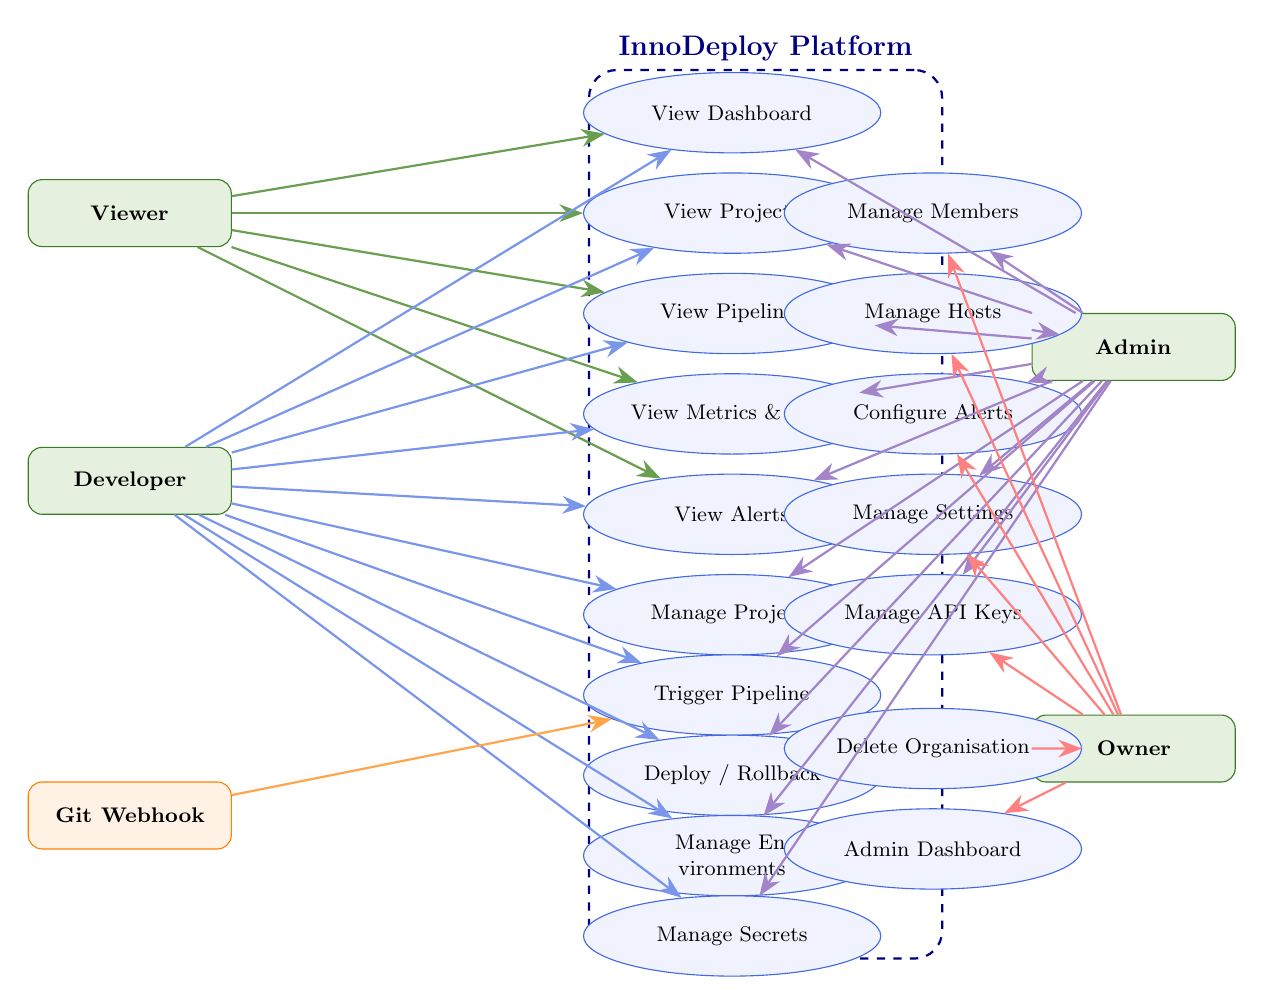
\begin{tikzpicture}[node distance=0.6cm and 2.5cm, scale=0.85, transform shape]

  % Actors
  \node[actor] (viewer) at (-7, 0) {Viewer};
  \node[actor] (dev) at (-7, -4) {Developer};
  \node[actor] (admin) at (8, -2) {Admin};
  \node[actor] (owner) at (8, -8) {Owner};
  \node[actor, fill=orange!10, draw=orange] (webhook) at (-7, -9) {Git Webhook};

  % System boundary
  \node[draw=NavyBlue, dashed, thick, rounded corners=10pt,
        fit={(0,-11) (5,2)},
        label={[font=\large\bfseries\color{NavyBlue}]above:InnoDeploy Platform}] (sys) {};

  % Use cases
  \node[usecase] (uc1) at (2, 1.5) {View Dashboard};
  \node[usecase] (uc2) at (2, 0) {View Projects};
  \node[usecase] (uc3) at (2, -1.5) {View Pipelines};
  \node[usecase] (uc4) at (2, -3) {View Metrics \& Logs};
  \node[usecase] (uc5) at (2, -4.5) {View Alerts};

  \node[usecase] (uc6) at (2, -6) {Manage Projects};
  \node[usecase] (uc7) at (2, -7.2) {Trigger Pipeline};
  \node[usecase] (uc8) at (2, -8.4) {Deploy / Rollback};
  \node[usecase] (uc9) at (2, -9.6) {Manage Environments};
  \node[usecase] (uc10) at (2, -10.8) {Manage Secrets};

  % Admin use cases (right side)
  \node[usecase] at (5, 0) (uc11) {Manage Members};
  \node[usecase] at (5, -1.5) (uc12) {Manage Hosts};
  \node[usecase] at (5, -3) (uc13) {Configure Alerts};
  \node[usecase] at (5, -4.5) (uc14) {Manage Settings};
  \node[usecase] at (5, -6) (uc15) {Manage API Keys};

  % Owner use cases
  \node[usecase] at (5, -8) (uc16) {Delete Organisation};
  \node[usecase] at (5, -9.5) (uc17) {Admin Dashboard};

  % Viewer connections
  \foreach \i in {1,2,3,4,5}
    \draw[arrow, OliveGreen!70] (viewer) -- (uc\i);

  % Developer connections
  \foreach \i in {1,2,3,4,5,6,7,8,9,10}
    \draw[arrow, RoyalBlue!70] (dev) -- (uc\i);

  % Admin connections
  \foreach \i in {1,2,3,4,5,6,7,8,9,10,11,12,13,14,15}
    \draw[arrow, RoyalPurple!50] (admin) -- (uc\i);

  % Owner connections
  \foreach \i in {11,12,13,14,15,16,17}
    \draw[arrow, red!50] (owner) -- (uc\i);

  % Webhook connection
  \draw[arrow, orange!70] (webhook) -- (uc7);

\end{tikzpicture}
\caption{Global Use Case Diagram}
\label{fig:usecase-global}
\end{figure}

\section{Detailed Use Cases}

\subsection{Use Case: Trigger Pipeline Run}

\begin{table}[H]
\centering
\caption{Use Case: Trigger Pipeline Run}
\begin{tabularx}{\textwidth}{l|X}
\toprule
\textbf{Use Case} & Trigger Pipeline Run \\
\midrule
\textbf{Actor} & Developer, Admin, Owner, Git Webhook \\
\textbf{Precondition} & Project exists; user has developer+ role; or valid webhook signature \\
\textbf{Main Flow} & 1. Actor selects project and provides pipeline parameters (version, strategy, branch, environment, steps). \\
& 2. System validates the request via Zod schema. \\
& 3. System creates a Pipeline document with status ``pending''. \\
& 4. System enqueues the job to the Redis pipeline queue. \\
& 5. Pipeline runner worker dequeues and executes steps sequentially in Docker containers. \\
& 6. System streams progress via SSE and WebSocket. \\
& 7. On completion, system updates Pipeline status to ``success'' or ``failed''. \\
\textbf{Postcondition} & Pipeline run recorded with step-level outputs and durations. \\
\textbf{Alternative} & A1: Validation fails $\rightarrow$ return 400 with field errors. \\
& A2: User cancels $\rightarrow$ set status to ``cancelled'', skip remaining steps. \\
& A3: Step timeout $\rightarrow$ mark step as ``failed'', proceed based on retry config. \\
\bottomrule
\end{tabularx}
\end{table}

\subsection{Use Case: Register and Login}

\begin{table}[H]
\centering
\caption{Use Case: User Registration}
\begin{tabularx}{\textwidth}{l|X}
\toprule
\textbf{Use Case} & User Registration \\
\midrule
\textbf{Actor} & Unregistered User \\
\textbf{Precondition} & Email not already registered \\
\textbf{Main Flow} & 1. User provides name, email, password, and optional organisation name. \\
& 2. System validates input via Zod schema. \\
& 3. System hashes password with bcrypt (12 rounds). \\
& 4. System creates User document. \\
& 5. If organisation name provided, system creates Organisation and assigns user as owner. \\
& 6. System issues JWT access token and refresh token. \\
\textbf{Postcondition} & User account created; tokens stored client-side. \\
\textbf{Alternative} & A1: Email already exists $\rightarrow$ return 409 conflict. \\
& A2: Rate limit exceeded $\rightarrow$ return 429. \\
\bottomrule
\end{tabularx}
\end{table}


% ══════════════════════════════════════════════════════════════════════════
%  CHAPTER 4 – SYSTEM ARCHITECTURE
% ══════════════════════════════════════════════════════════════════════════
\chapter{System Architecture}

\section{Global Architecture Overview}

InnoDeploy follows a \textbf{microservices-inspired monorepo architecture} with clear separation between the API server, background workers, real-time gateway, and frontend client.

\begin{figure}[H]
\centering
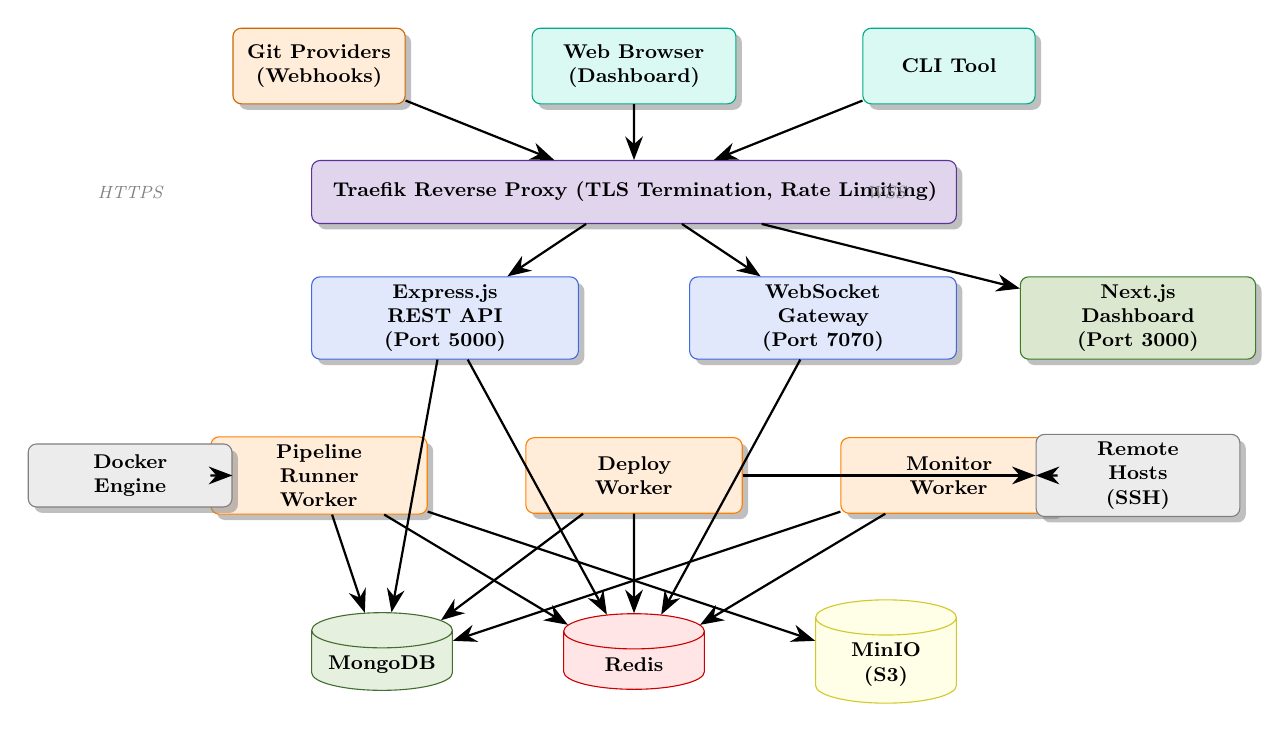
\begin{tikzpicture}[node distance=1.5cm and 2cm, scale=0.8, transform shape]

  % Client Layer
  \node[component, fill=innoprimary!15, draw=innoprimary!80!black, text width=3cm] (browser) at (0, 8) {Web Browser\\(Dashboard)};
  \node[component, fill=innoprimary!15, draw=innoprimary!80!black, text width=2.5cm] (cli) at (5, 8) {CLI Tool};
  \node[component, fill=orange!15, draw=orange!80!black, text width=2.5cm] (githubwh) at (-5, 8) {Git Providers\\(Webhooks)};

  % Reverse Proxy
  \node[component, fill=RoyalPurple!15, draw=RoyalPurple, text width=10cm, minimum height=1cm] (traefik) at (0, 6) {Traefik Reverse Proxy (TLS Termination, Rate Limiting)};

  % API Layer
  \node[component, fill=RoyalBlue!15, draw=RoyalBlue, text width=4cm] (api) at (-3, 4) {Express.js\\REST API\\(Port 5000)};
  \node[component, fill=RoyalBlue!15, draw=RoyalBlue, text width=4cm] (ws) at (3, 4) {WebSocket\\Gateway\\(Port 7070)};

  % Dashboard
  \node[component, fill=OliveGreen!15, draw=OliveGreen, text width=3.5cm] (dashboard) at (8, 4) {Next.js\\Dashboard\\(Port 3000)};

  % Worker Layer
  \node[component, fill=orange!15, draw=orange, text width=3.2cm] (prunner) at (-5, 1.5) {Pipeline\\Runner\\Worker};
  \node[component, fill=orange!15, draw=orange, text width=3.2cm] (dworker) at (0, 1.5) {Deploy\\Worker};
  \node[component, fill=orange!15, draw=orange, text width=3.2cm] (mworker) at (5, 1.5) {Monitor\\Worker};

  % Data Layer
  \node[database] (mongo) at (-4, -1.5) {MongoDB};
  \node[database, fill=red!10, draw=red!80!black] (redis) at (0, -1.5) {Redis};
  \node[database, fill=yellow!10, draw=yellow!80!black] (minio) at (4, -1.5) {MinIO\\(S3)};

  % External
  \node[server, fill=gray!15, draw=gray] (hosts) at (8, 1.5) {Remote\\Hosts\\(SSH)};
  \node[server, fill=gray!15, draw=gray] (docker) at (-8, 1.5) {Docker\\Engine};

  % Connections - Client to Traefik
  \draw[arrow] (browser) -- (traefik);
  \draw[arrow] (cli) -- (traefik);
  \draw[arrow] (githubwh) -- (traefik);

  % Traefik to services
  \draw[arrow] (traefik) -- (api);
  \draw[arrow] (traefik) -- (ws);
  \draw[arrow] (traefik) -- (dashboard);

  % API to data
  \draw[arrow] (api) -- (mongo);
  \draw[arrow] (api) -- (redis);

  % WebSocket to Redis
  \draw[arrow] (ws) -- (redis);

  % Workers to data
  \draw[arrow] (prunner) -- (mongo);
  \draw[arrow] (prunner) -- (redis);
  \draw[arrow] (dworker) -- (mongo);
  \draw[arrow] (dworker) -- (redis);
  \draw[arrow] (mworker) -- (mongo);
  \draw[arrow] (mworker) -- (redis);

  % Workers to external
  \draw[arrow] (prunner) -- (docker);
  \draw[arrow] (dworker) -- (hosts);
  \draw[arrow] (mworker) -- (hosts);
  \draw[arrow] (prunner) -- (minio);

  % Labels
  \node[font=\footnotesize\itshape, gray] at (-8, 6) {HTTPS};
  \node[font=\footnotesize\itshape, gray] at (4, 6) {WSS};

\end{tikzpicture}
\caption{Global System Architecture}
\label{fig:global-arch}
\end{figure}

\section{Technology Stack}

\begin{table}[H]
\centering
\caption{Technology Stack}
\label{tab:techstack}
\begin{tabularx}{\textwidth}{l|l|X}
\toprule
\textbf{Layer} & \textbf{Technology} & \textbf{Role} \\
\midrule
\multirow{8}{*}{\textbf{Frontend}} & Next.js 15 & Server-side rendering, routing, and API integration \\
& React 19 & Component-based UI framework \\
& TypeScript 5.5 & Static type safety \\
& Tailwind CSS 3.4 & Utility-first CSS framework \\
& Zustand 4.5 & Lightweight state management \\
& React Query 5.51 & Server state caching and synchronization \\
& Recharts 2.15 & Data visualization charts \\
& xterm.js 5.3 & Terminal emulator for log viewing \\
\midrule
\multirow{8}{*}{\textbf{Backend}} & Express.js 4.21 & HTTP REST API framework \\
& Mongoose 8.5 & MongoDB ODM with schema validation \\
& Redis 4.7 & Caching, token storage, pub/sub, job queues \\
& BullMQ 5.71 & Persistent job queue management \\
& Dockerode 4.0 & Docker Engine API client \\
& SSH2 1.17 & SSH client for remote host access \\
& Zod 4.3 & Runtime schema validation \\
& JSON Web Token 9.0 & Stateless authentication tokens \\
\midrule
\multirow{4}{*}{\textbf{Infrastructure}} & Docker \& Compose & Container orchestration \\
& Traefik 3.1 & Reverse proxy with auto-TLS \\
& MongoDB 7 & Document database \\
& MinIO & S3-compatible object storage \\
\midrule
\textbf{CLI} & Commander.js & CLI argument parsing and subcommands \\
\bottomrule
\end{tabularx}
\end{table}

\section{Component Architecture}

\subsection{Backend Components}

The backend is organised into the following layers:

\begin{figure}[H]
\centering
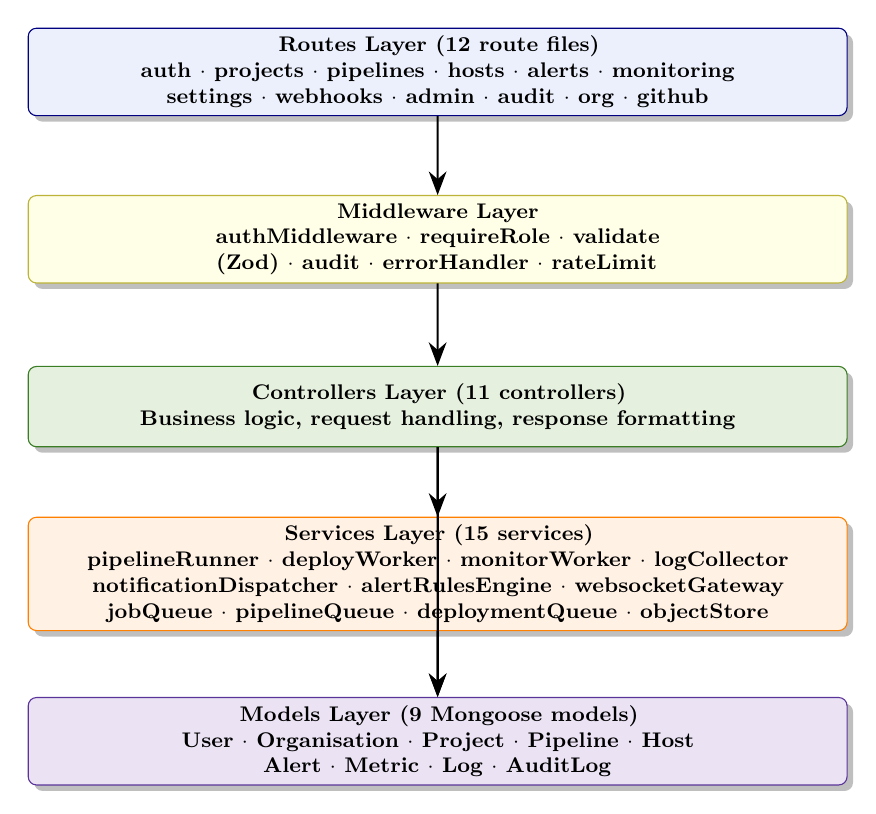
\begin{tikzpicture}[node distance=1cm, scale=0.85, transform shape]

  % Routes layer
  \node[component, text width=12cm, fill=RoyalBlue!10] (routes) at (0, 6) {
    \textbf{Routes Layer} (12 route files)\\
    auth $\cdot$ projects $\cdot$ pipelines $\cdot$ hosts $\cdot$ alerts $\cdot$ monitoring\\
    settings $\cdot$ webhooks $\cdot$ admin $\cdot$ audit $\cdot$ org $\cdot$ github
  };

  % Middleware layer
  \node[component, text width=12cm, fill=yellow!10, draw=yellow!70!black] (middleware) at (0, 3.5) {
    \textbf{Middleware Layer}\\
    authMiddleware $\cdot$ requireRole $\cdot$ validate (Zod) $\cdot$ audit $\cdot$ errorHandler $\cdot$ rateLimit
  };

  % Controllers layer
  \node[component, text width=12cm, fill=OliveGreen!10, draw=OliveGreen] (controllers) at (0, 1) {
    \textbf{Controllers Layer} (11 controllers)\\
    Business logic, request handling, response formatting
  };

  % Services layer
  \node[component, text width=12cm, fill=orange!10, draw=orange] (services) at (0, -1.5) {
    \textbf{Services Layer} (15 services)\\
    pipelineRunner $\cdot$ deployWorker $\cdot$ monitorWorker $\cdot$ logCollector\\
    notificationDispatcher $\cdot$ alertRulesEngine $\cdot$ websocketGateway\\
    jobQueue $\cdot$ pipelineQueue $\cdot$ deploymentQueue $\cdot$ objectStore
  };

  % Models layer
  \node[component, text width=12cm, fill=RoyalPurple!10, draw=RoyalPurple] (models) at (0, -4) {
    \textbf{Models Layer} (9 Mongoose models)\\
    User $\cdot$ Organisation $\cdot$ Project $\cdot$ Pipeline $\cdot$ Host\\
    Alert $\cdot$ Metric $\cdot$ Log $\cdot$ AuditLog
  };

  % Arrows
  \draw[arrow] (routes) -- (middleware);
  \draw[arrow] (middleware) -- (controllers);
  \draw[arrow] (controllers) -- (services);
  \draw[arrow] (controllers) -- (models);
  \draw[arrow] (services) -- (models);

\end{tikzpicture}
\caption{Backend Layered Architecture}
\label{fig:backend-layers}
\end{figure}

\subsection{Frontend Architecture}

The Next.js dashboard follows a page-based routing architecture:

\begin{figure}[H]
\centering
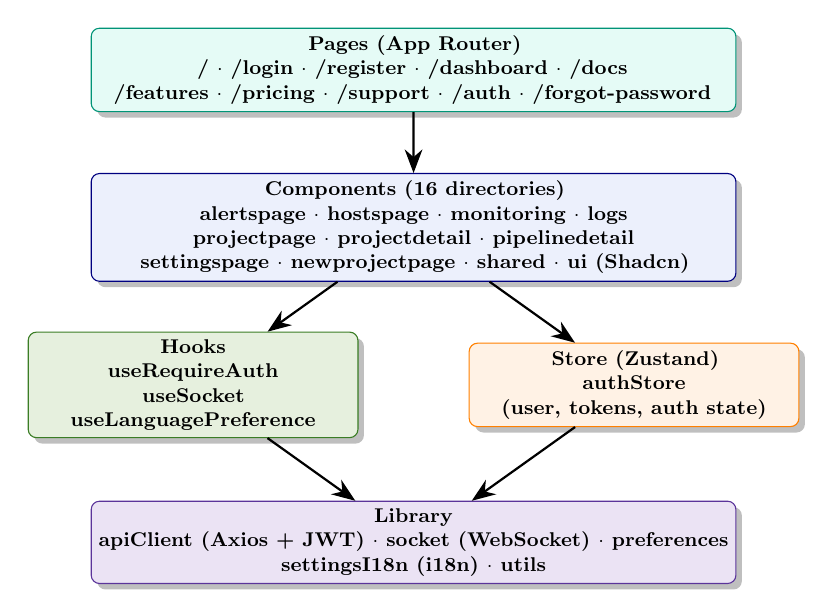
\begin{tikzpicture}[node distance=0.8cm, scale=0.8, transform shape]

  \node[component, text width=10cm, fill=innoprimary!10, draw=innoprimary!70!black] (pages) at (0, 5) {
    \textbf{Pages (App Router)}\\
    / $\cdot$ /login $\cdot$ /register $\cdot$ /dashboard $\cdot$ /docs\\
    /features $\cdot$ /pricing $\cdot$ /support $\cdot$ /auth $\cdot$ /forgot-password
  };

  \node[component, text width=10cm, fill=RoyalBlue!10] (components) at (0, 2.5) {
    \textbf{Components} (16 directories)\\
    alertspage $\cdot$ hostspage $\cdot$ monitoring $\cdot$ logs\\
    projectpage $\cdot$ projectdetail $\cdot$ pipelinedetail\\
    settingspage $\cdot$ newprojectpage $\cdot$ shared $\cdot$ ui (Shadcn)
  };

  \node[component, text width=5cm, fill=OliveGreen!10, draw=OliveGreen] (hooks) at (-3.5, 0) {
    \textbf{Hooks}\\
    useRequireAuth\\
    useSocket\\
    useLanguagePreference
  };

  \node[component, text width=5cm, fill=orange!10, draw=orange] (store) at (3.5, 0) {
    \textbf{Store (Zustand)}\\
    authStore\\
    (user, tokens, auth state)
  };

  \node[component, text width=10cm, fill=RoyalPurple!10, draw=RoyalPurple] (lib) at (0, -2.5) {
    \textbf{Library}\\
    apiClient (Axios + JWT) $\cdot$ socket (WebSocket) $\cdot$ preferences\\
    settingsI18n (i18n) $\cdot$ utils
  };

  \draw[arrow] (pages) -- (components);
  \draw[arrow] (components) -- (hooks);
  \draw[arrow] (components) -- (store);
  \draw[arrow] (hooks) -- (lib);
  \draw[arrow] (store) -- (lib);

\end{tikzpicture}
\caption{Frontend Component Architecture}
\label{fig:frontend-arch}
\end{figure}

\section{Multi-Tenancy Architecture}

InnoDeploy implements \textbf{organisation-level multi-tenancy} where all resources are scoped to an organisation:

\begin{itemize}[noitemsep]
  \item Each \textbf{User} belongs to exactly one \textbf{Organisation}.
  \item Each \textbf{Project}, \textbf{Host}, and \textbf{AuditLog} is scoped to an \texttt{organisationId}.
  \item \textbf{Pipelines}, \textbf{Alerts}, \textbf{Metrics}, and \textbf{Logs} are scoped via their parent \texttt{projectId}.
  \item The middleware chain validates organisation membership before allowing access.
  \item Plan limits (maxProjects, maxDeploysPerMonth, maxMembers) are enforced at the organisation level.
\end{itemize}

\section{Real-Time Communication Architecture}

\begin{figure}[H]
\centering
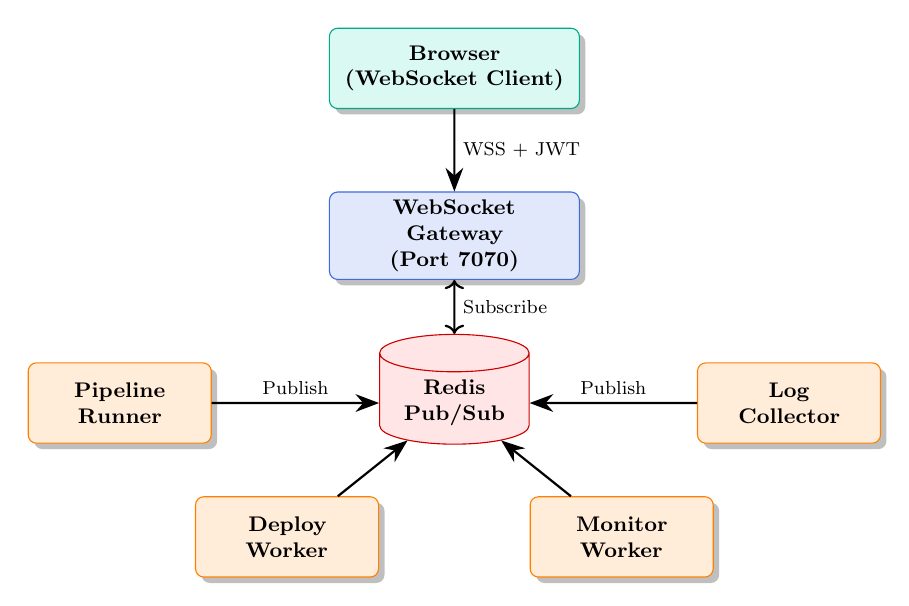
\begin{tikzpicture}[node distance=1.5cm and 2cm, scale=0.85, transform shape]

  \node[component, fill=innoprimary!15, draw=innoprimary!80!black] (client) at (0, 4) {Browser\\(WebSocket Client)};
  \node[component, fill=RoyalBlue!15, draw=RoyalBlue] (gateway) at (0, 1.5) {WebSocket\\Gateway\\(Port 7070)};
  \node[database, fill=red!10, draw=red!80!black] (redis) at (0, -1) {Redis\\Pub/Sub};

  \node[component, fill=orange!15, draw=orange, text width=2.5cm] (pr) at (-5, -1) {Pipeline\\Runner};
  \node[component, fill=orange!15, draw=orange, text width=2.5cm] (dw) at (-2.5, -3) {Deploy\\Worker};
  \node[component, fill=orange!15, draw=orange, text width=2.5cm] (mw) at (2.5, -3) {Monitor\\Worker};
  \node[component, fill=orange!15, draw=orange, text width=2.5cm] (lc) at (5, -1) {Log\\Collector};

  \draw[arrow] (client) -- node[right, font=\footnotesize] {WSS + JWT} (gateway);
  \draw[arrow, <->] (gateway) -- node[right, font=\footnotesize] {Subscribe} (redis);
  \draw[arrow] (pr) -- node[above, font=\footnotesize] {Publish} (redis);
  \draw[arrow] (dw) -- (redis);
  \draw[arrow] (mw) -- (redis);
  \draw[arrow] (lc) -- node[above, font=\footnotesize] {Publish} (redis);

\end{tikzpicture}
\caption{Real-Time Communication via Redis Pub/Sub}
\label{fig:realtime-arch}
\end{figure}

The WebSocket gateway supports the following channel subscriptions:
\begin{itemize}[noitemsep]
  \item \texttt{monitoring:stream}, \texttt{monitoring:project:\{id\}} -- real-time metrics
  \item \texttt{pipeline:events}, \texttt{pipeline:logs:\{id\}} -- pipeline progress
  \item \texttt{deploy:events} -- deployment status updates
  \item \texttt{logs:stream}, \texttt{logs:project:\{id\}} -- container log streaming
\end{itemize}


% ══════════════════════════════════════════════════════════════════════════
%  CHAPTER 5 – DATA MODELLING
% ══════════════════════════════════════════════════════════════════════════
\chapter{Data Modelling}

\section{Class Diagram}

The following UML class diagram represents the complete data model of the InnoDeploy platform. The system uses MongoDB as its primary database with Mongoose ODM for schema enforcement.

\begin{figure}[H]
\centering
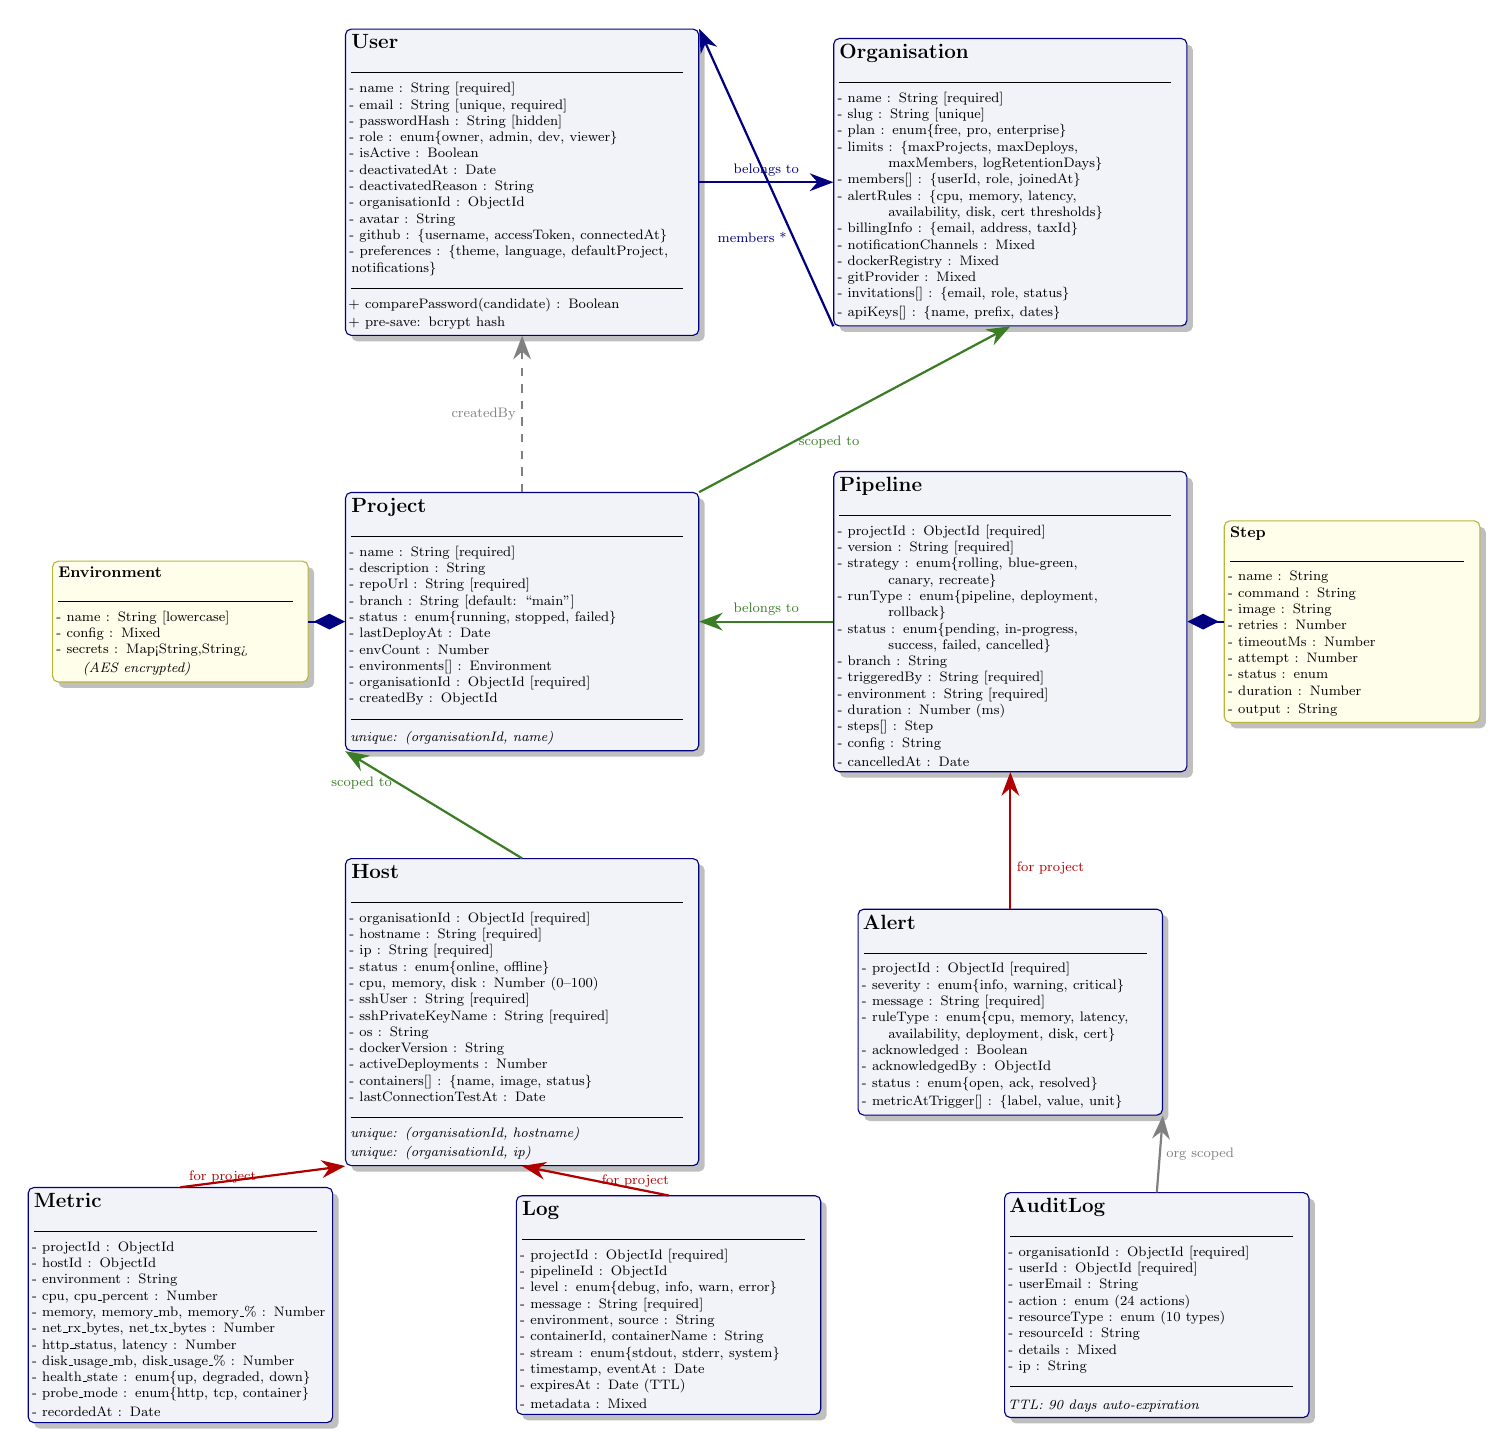
\begin{tikzpicture}[scale=0.62, transform shape]

  % ── User ───────────────────────────────────
  \node[classbox, text width=7cm] (user) at (0, 0) {
    \textbf{\large User}\\[3pt]
    \rule{6.8cm}{0.4pt}\\[2pt]
    \footnotesize
    - name : String [required]\\
    - email : String [unique, required]\\
    - passwordHash : String [hidden]\\
    - role : enum\{owner, admin, dev, viewer\}\\
    - isActive : Boolean\\
    - deactivatedAt : Date\\
    - deactivatedReason : String\\
    - organisationId : ObjectId\\
    - avatar : String\\
    - github : \{username, accessToken, connectedAt\}\\
    - preferences : \{theme, language, defaultProject, notifications\}\\
    \rule{6.8cm}{0.4pt}\\[2pt]
    + comparePassword(candidate) : Boolean\\
    + pre-save: bcrypt hash
  };

  % ── Organisation ───────────────────────────
  \node[classbox, text width=7cm] (org) at (10, 0) {
    \textbf{\large Organisation}\\[3pt]
    \rule{6.8cm}{0.4pt}\\[2pt]
    \footnotesize
    - name : String [required]\\
    - slug : String [unique]\\
    - plan : enum\{free, pro, enterprise\}\\
    - limits : \{maxProjects, maxDeploys,\\
    \hspace{1cm}maxMembers, logRetentionDays\}\\
    - members[] : \{userId, role, joinedAt\}\\
    - alertRules : \{cpu, memory, latency,\\
    \hspace{1cm}availability, disk, cert thresholds\}\\
    - billingInfo : \{email, address, taxId\}\\
    - notificationChannels : Mixed\\
    - dockerRegistry : Mixed\\
    - gitProvider : Mixed\\
    - invitations[] : \{email, role, status\}\\
    - apiKeys[] : \{name, prefix, dates\}
  };

  % ── Project ────────────────────────────────
  \node[classbox, text width=7cm] (project) at (0, -9) {
    \textbf{\large Project}\\[3pt]
    \rule{6.8cm}{0.4pt}\\[2pt]
    \footnotesize
    - name : String [required]\\
    - description : String\\
    - repoUrl : String [required]\\
    - branch : String [default: ``main'']\\
    - status : enum\{running, stopped, failed\}\\
    - lastDeployAt : Date\\
    - envCount : Number\\
    - environments[] : Environment\\
    - organisationId : ObjectId [required]\\
    - createdBy : ObjectId\\
    \rule{6.8cm}{0.4pt}\\[2pt]
    \textit{unique: (organisationId, name)}
  };

  % ── Environment (embedded) ─────────────────
  \node[classbox, text width=5cm, fill=yellow!8, draw=yellow!70!black] (env) at (-7, -9) {
    \textbf{Environment}\\[3pt]
    \rule{4.8cm}{0.4pt}\\[2pt]
    \footnotesize
    - name : String [lowercase]\\
    - config : Mixed\\
    - secrets : Map<String,String>\\
    \hspace{0.5cm}\textit{(AES encrypted)}
  };

  % ── Pipeline ───────────────────────────────
  \node[classbox, text width=7cm] (pipeline) at (10, -9) {
    \textbf{\large Pipeline}\\[3pt]
    \rule{6.8cm}{0.4pt}\\[2pt]
    \footnotesize
    - projectId : ObjectId [required]\\
    - version : String [required]\\
    - strategy : enum\{rolling, blue-green,\\
    \hspace{1cm}canary, recreate\}\\
    - runType : enum\{pipeline, deployment,\\
    \hspace{1cm}rollback\}\\
    - status : enum\{pending, in-progress,\\
    \hspace{1cm}success, failed, cancelled\}\\
    - branch : String\\
    - triggeredBy : String [required]\\
    - environment : String [required]\\
    - duration : Number (ms)\\
    - steps[] : Step\\
    - config : String\\
    - cancelledAt : Date
  };

  % ── Step (embedded) ────────────────────────
  \node[classbox, text width=5cm, fill=yellow!8, draw=yellow!70!black] (step) at (17, -9) {
    \textbf{Step}\\[3pt]
    \rule{4.8cm}{0.4pt}\\[2pt]
    \footnotesize
    - name : String\\
    - command : String\\
    - image : String\\
    - retries : Number\\
    - timeoutMs : Number\\
    - attempt : Number\\
    - status : enum\\
    - duration : Number\\
    - output : String
  };

  % ── Host ───────────────────────────────────
  \node[classbox, text width=7cm] (host) at (0, -17) {
    \textbf{\large Host}\\[3pt]
    \rule{6.8cm}{0.4pt}\\[2pt]
    \footnotesize
    - organisationId : ObjectId [required]\\
    - hostname : String [required]\\
    - ip : String [required]\\
    - status : enum\{online, offline\}\\
    - cpu, memory, disk : Number (0--100)\\
    - sshUser : String [required]\\
    - sshPrivateKeyName : String [required]\\
    - os : String\\
    - dockerVersion : String\\
    - activeDeployments : Number\\
    - containers[] : \{name, image, status\}\\
    - lastConnectionTestAt : Date\\
    \rule{6.8cm}{0.4pt}\\[2pt]
    \textit{unique: (organisationId, hostname)}\\
    \textit{unique: (organisationId, ip)}
  };

  % ── Alert ──────────────────────────────────
  \node[classbox, text width=6cm] (alert) at (10, -17) {
    \textbf{\large Alert}\\[3pt]
    \rule{5.8cm}{0.4pt}\\[2pt]
    \footnotesize
    - projectId : ObjectId [required]\\
    - severity : enum\{info, warning, critical\}\\
    - message : String [required]\\
    - ruleType : enum\{cpu, memory, latency,\\
    \hspace{0.5cm}availability, deployment, disk, cert\}\\
    - acknowledged : Boolean\\
    - acknowledgedBy : ObjectId\\
    - status : enum\{open, ack, resolved\}\\
    - metricAtTrigger[] : \{label, value, unit\}
  };

  % ── Metric ─────────────────────────────────
  \node[classbox, text width=6cm] (metric) at (-7, -23) {
    \textbf{\large Metric}\\[3pt]
    \rule{5.8cm}{0.4pt}\\[2pt]
    \footnotesize
    - projectId : ObjectId\\
    - hostId : ObjectId\\
    - environment : String\\
    - cpu, cpu\_percent : Number\\
    - memory, memory\_mb, memory\_\% : Number\\
    - net\_rx\_bytes, net\_tx\_bytes : Number\\
    - http\_status, latency : Number\\
    - disk\_usage\_mb, disk\_usage\_\% : Number\\
    - health\_state : enum\{up, degraded, down\}\\
    - probe\_mode : enum\{http, tcp, container\}\\
    - recordedAt : Date
  };

  % ── Log ────────────────────────────────────
  \node[classbox, text width=6cm] (log) at (3, -23) {
    \textbf{\large Log}\\[3pt]
    \rule{5.8cm}{0.4pt}\\[2pt]
    \footnotesize
    - projectId : ObjectId [required]\\
    - pipelineId : ObjectId\\
    - level : enum\{debug, info, warn, error\}\\
    - message : String [required]\\
    - environment, source : String\\
    - containerId, containerName : String\\
    - stream : enum\{stdout, stderr, system\}\\
    - timestamp, eventAt : Date\\
    - expiresAt : Date (TTL)\\
    - metadata : Mixed
  };

  % ── AuditLog ───────────────────────────────
  \node[classbox, text width=6cm] (audit) at (13, -23) {
    \textbf{\large AuditLog}\\[3pt]
    \rule{5.8cm}{0.4pt}\\[2pt]
    \footnotesize
    - organisationId : ObjectId [required]\\
    - userId : ObjectId [required]\\
    - userEmail : String\\
    - action : enum (24 actions)\\
    - resourceType : enum (10 types)\\
    - resourceId : String\\
    - details : Mixed\\
    - ip : String\\
    \rule{5.8cm}{0.4pt}\\[2pt]
    \textit{TTL: 90 days auto-expiration}
  };

  % ── Relationships ──────────────────────────
  % User -> Organisation
  \draw[arrow, thick, NavyBlue] (user.east) -- node[above, font=\footnotesize] {belongs to} (org.west);
  \draw[arrow, thick, NavyBlue] (org.south west) -- node[left, font=\footnotesize, pos=0.3] {members *} (user.north east);

  % Project -> Organisation
  \draw[arrow, thick, OliveGreen] (project.north east) -- node[right, font=\footnotesize, pos=0.3] {scoped to} (org.south);

  % Project -> User (createdBy)
  \draw[dashedarrow, gray] (project.north) -- node[left, font=\footnotesize] {createdBy} (user.south);

  % Environment <- Project (composition)
  \draw[thick, NavyBlue, -{Diamond[fill=NavyBlue, length=4mm]}] (env.east) -- (project.west);

  % Pipeline -> Project
  \draw[arrow, thick, OliveGreen] (pipeline.west) -- node[above, font=\footnotesize] {belongs to} (project.east);

  % Step <- Pipeline (composition)
  \draw[thick, NavyBlue, -{Diamond[fill=NavyBlue, length=4mm]}] (step.west) -- (pipeline.east);

  % Host -> Organisation
  \draw[arrow, thick, OliveGreen] (host.north) -- node[left, font=\footnotesize, pos=0.7] {scoped to} (project.south west);

  % Alert -> Project
  \draw[arrow, thick, red!70!black] (alert.north) -- node[right, font=\footnotesize, pos=0.3] {for project} (pipeline.south);

  % Metric -> Project
  \draw[arrow, thick, red!70!black] (metric.north) -- node[left, font=\footnotesize] {for project} (host.south west);

  % Log -> Project
  \draw[arrow, thick, red!70!black] (log.north) -- node[right, font=\footnotesize, pos=0.5] {for project} (host.south);

  % AuditLog -> Organisation
  \draw[arrow, thick, gray] (audit.north) -- node[right, font=\footnotesize, pos=0.5] {org scoped} (alert.south east);

\end{tikzpicture}
\caption{Complete UML Class Diagram}
\label{fig:class-diagram}
\end{figure}

\section{Data Model Families}

The models can be categorised into three domain families:

\begin{description}[style=nextline]
  \item[\textbf{Identity Domain}] \texttt{User}, \texttt{Organisation} -- Authentication, authorisation, and multi-tenancy.
  \item[\textbf{Delivery Domain}] \texttt{Project}, \texttt{Pipeline}, \texttt{Host} -- CI/CD pipeline execution and deployment orchestration.
  \item[\textbf{Observability Domain}] \texttt{Alert}, \texttt{Metric}, \texttt{Log}, \texttt{AuditLog} -- Monitoring, alerting, logging, and audit trail.
\end{description}

\section{Database Indexing Strategy}

\begin{table}[H]
\centering
\caption{Key Database Indexes}
\label{tab:indexes}
\begin{tabularx}{\textwidth}{l|l|X}
\toprule
\textbf{Collection} & \textbf{Index} & \textbf{Purpose} \\
\midrule
Project & (organisationId, name) unique & Prevent duplicate project names per org \\
Host & (organisationId, hostname) unique & Prevent duplicate hostnames per org \\
Host & (organisationId, ip) unique & Prevent duplicate IPs per org \\
AuditLog & (organisationId, createdAt desc) & Fast audit log queries \\
AuditLog & expiresAt TTL & 90-day auto-expiration \\
Log & (projectId, eventAt desc) & Chronological log queries \\
Log & (projectId, level, eventAt desc) & Level-filtered log queries \\
Log & text(message, source, containerName) & Full-text search \\
Log & expiresAt TTL & Configurable log retention \\
\bottomrule
\end{tabularx}
\end{table}


% ══════════════════════════════════════════════════════════════════════════
%  CHAPTER 6 – DETAILED DESIGN (SEQUENCE DIAGRAMS)
% ══════════════════════════════════════════════════════════════════════════
\chapter{Detailed Design}

\section{Authentication Flow -- Login Sequence}

\begin{figure}[H]
\centering
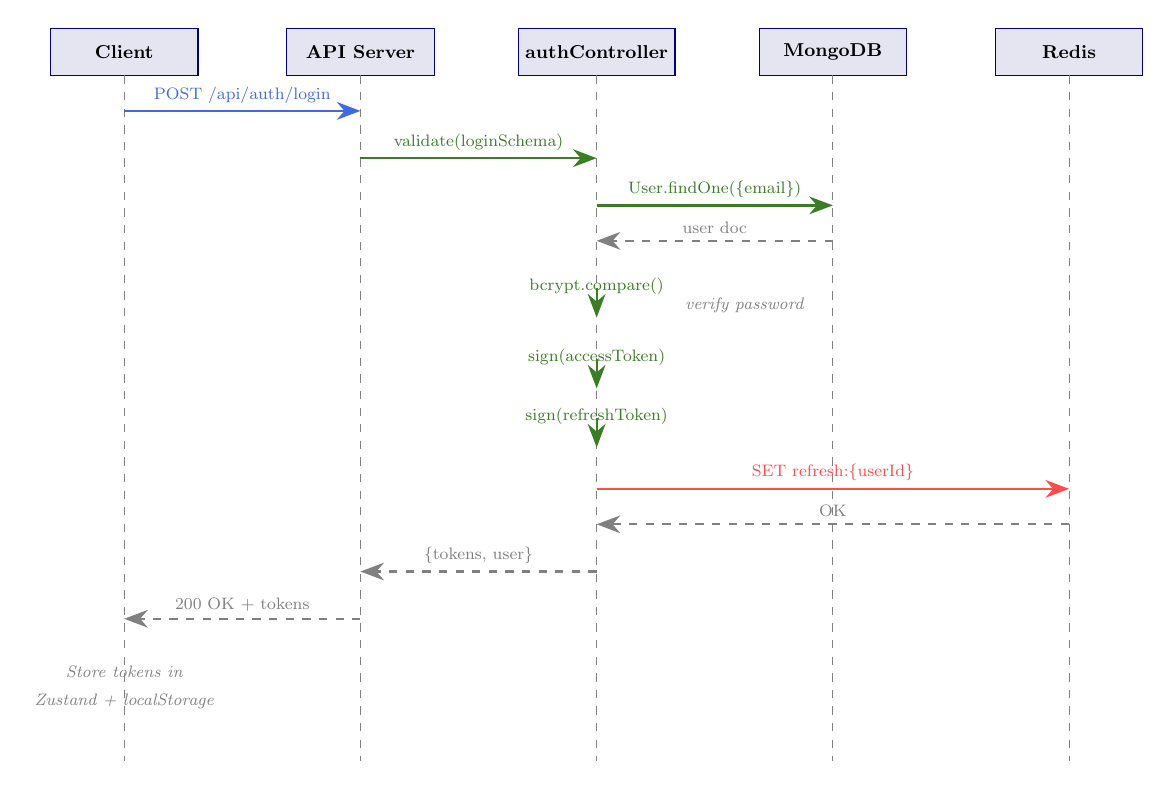
\begin{tikzpicture}[scale=0.75, transform shape]

  % Objects
  \node[seqobj] (client) at (0, 0) {Client};
  \node[seqobj] (api) at (4, 0) {API Server};
  \node[seqobj] (auth) at (8, 0) {authController};
  \node[seqobj] (db) at (12, 0) {MongoDB};
  \node[seqobj] (red) at (16, 0) {Redis};

  % Lifelines
  \foreach \x in {0, 4, 8, 12, 16}
    \draw[dashed, gray] (\x, -0.4) -- (\x, -12);

  % Messages
  \draw[arrow, RoyalBlue] (0, -1) -- node[above, font=\footnotesize] {POST /api/auth/login} (4, -1);
  \draw[arrow, OliveGreen] (4, -1.8) -- node[above, font=\footnotesize] {validate(loginSchema)} (8, -1.8);
  \draw[arrow, OliveGreen] (8, -2.6) -- node[above, font=\footnotesize] {User.findOne(\{email\})} (12, -2.6);
  \draw[dashedarrow, gray] (12, -3.2) -- node[above, font=\footnotesize] {user doc} (8, -3.2);

  \draw[arrow, OliveGreen] (8, -4) -- node[above, font=\footnotesize] {bcrypt.compare()} (8, -4.5);
  \node[font=\footnotesize\itshape, gray] at (10.5, -4.3) {verify password};

  \draw[arrow, OliveGreen] (8, -5.2) -- node[above, font=\footnotesize] {sign(accessToken)} (8, -5.7);
  \draw[arrow, OliveGreen] (8, -6.2) -- node[above, font=\footnotesize] {sign(refreshToken)} (8, -6.7);

  \draw[arrow, red!70] (8, -7.4) -- node[above, font=\footnotesize] {SET refresh:\{userId\}} (16, -7.4);
  \draw[dashedarrow, gray] (16, -8) -- node[above, font=\footnotesize] {OK} (8, -8);

  \draw[dashedarrow, gray] (8, -8.8) -- node[above, font=\footnotesize] {\{tokens, user\}} (4, -8.8);
  \draw[dashedarrow, gray] (4, -9.6) -- node[above, font=\footnotesize] {200 OK + tokens} (0, -9.6);

  \node[font=\footnotesize\itshape, gray] at (0, -10.5) {Store tokens in};
  \node[font=\footnotesize\itshape, gray] at (0, -11) {Zustand + localStorage};

\end{tikzpicture}
\caption{Login Authentication Sequence Diagram}
\label{fig:seq-login}
\end{figure}

\section{Pipeline Execution Flow}

\begin{figure}[H]
\centering
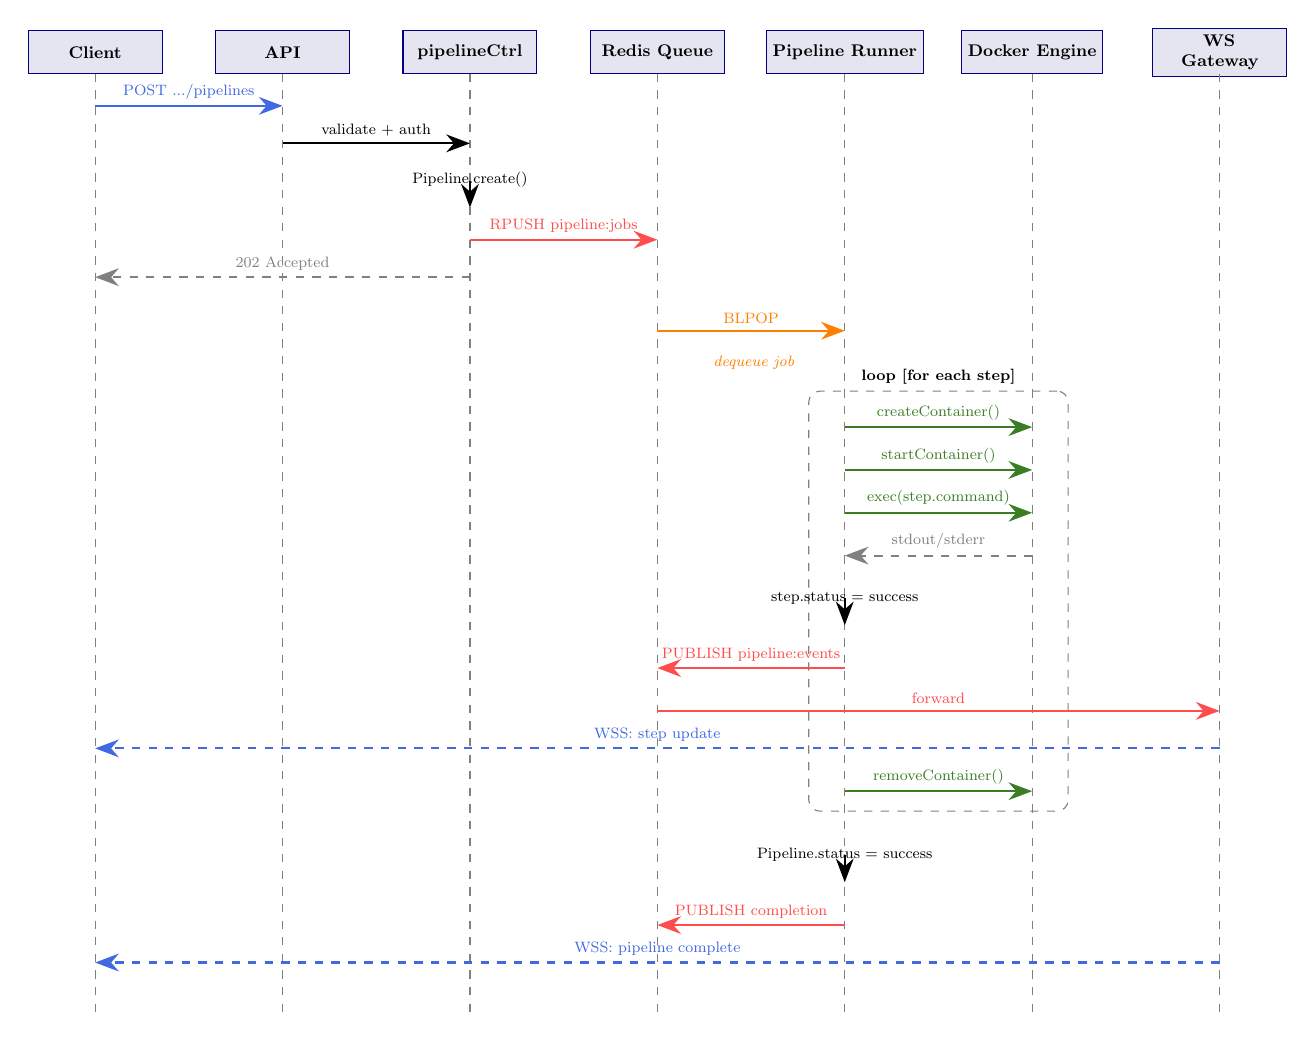
\begin{tikzpicture}[scale=0.68, transform shape]

  % Objects
  \node[seqobj] (client) at (0, 0) {Client};
  \node[seqobj] (api) at (3.5, 0) {API};
  \node[seqobj] (ctrl) at (7, 0) {pipelineCtrl};
  \node[seqobj] (queue) at (10.5, 0) {Redis Queue};
  \node[seqobj] (runner) at (14, 0) {Pipeline Runner};
  \node[seqobj] (docker) at (17.5, 0) {Docker Engine};
  \node[seqobj, text width=1.5cm] (ws) at (21, 0) {WS Gateway};

  % Lifelines
  \foreach \x in {0, 3.5, 7, 10.5, 14, 17.5, 21}
    \draw[dashed, gray] (\x, -0.4) -- (\x, -18);

  % Trigger
  \draw[arrow, RoyalBlue] (0, -1) -- node[above, font=\footnotesize] {POST .../pipelines} (3.5, -1);
  \draw[arrow] (3.5, -1.7) -- node[above, font=\footnotesize] {validate + auth} (7, -1.7);
  \draw[arrow] (7, -2.4) -- node[above, font=\footnotesize] {Pipeline.create()} (7, -2.9);
  \draw[arrow, red!70] (7, -3.5) -- node[above, font=\footnotesize] {RPUSH pipeline:jobs} (10.5, -3.5);
  \draw[dashedarrow, gray] (7, -4.2) -- node[above, font=\footnotesize] {202 Accepted} (0, -4.2);

  % Worker picks up
  \draw[arrow, orange] (10.5, -5.2) -- node[above, font=\footnotesize] {BLPOP} (14, -5.2);
  \node[font=\footnotesize\itshape, orange] at (12.3, -5.8) {dequeue job};

  % For each step
  \node[draw=gray, dashed, rounded corners, fit={([xshift=-0.5cm]14, -6.5) ([xshift=0.5cm]17.5, -14)}, label={[font=\footnotesize\bfseries]above:loop [for each step]}] {};

  \draw[arrow, OliveGreen] (14, -7) -- node[above, font=\footnotesize] {createContainer()} (17.5, -7);
  \draw[arrow, OliveGreen] (14, -7.8) -- node[above, font=\footnotesize] {startContainer()} (17.5, -7.8);
  \draw[arrow, OliveGreen] (14, -8.6) -- node[above, font=\footnotesize] {exec(step.command)} (17.5, -8.6);
  \draw[dashedarrow, gray] (17.5, -9.4) -- node[above, font=\footnotesize] {stdout/stderr} (14, -9.4);

  % Update status
  \draw[arrow] (14, -10.2) -- node[above, font=\footnotesize] {step.status = success} (14, -10.7);
  \draw[arrow, red!70] (14, -11.5) -- node[above, font=\footnotesize] {PUBLISH pipeline:events} (10.5, -11.5);
  \draw[arrow, red!70] (10.5, -12.3) -- node[above, font=\footnotesize] {forward} (21, -12.3);
  \draw[dashedarrow, RoyalBlue] (21, -13) -- node[above, font=\footnotesize] {WSS: step update} (0, -13);

  % Cleanup
  \draw[arrow, OliveGreen] (14, -13.8) -- node[above, font=\footnotesize] {removeContainer()} (17.5, -13.8);

  % Final
  \draw[arrow] (14, -15) -- node[above, font=\footnotesize] {Pipeline.status = success} (14, -15.5);
  \draw[arrow, red!70] (14, -16.3) -- node[above, font=\footnotesize] {PUBLISH completion} (10.5, -16.3);
  \draw[dashedarrow, RoyalBlue] (21, -17) -- node[above, font=\footnotesize] {WSS: pipeline complete} (0, -17);

\end{tikzpicture}
\caption{Pipeline Execution Sequence Diagram}
\label{fig:seq-pipeline}
\end{figure}

\section{Deployment Flow}

\begin{figure}[H]
\centering
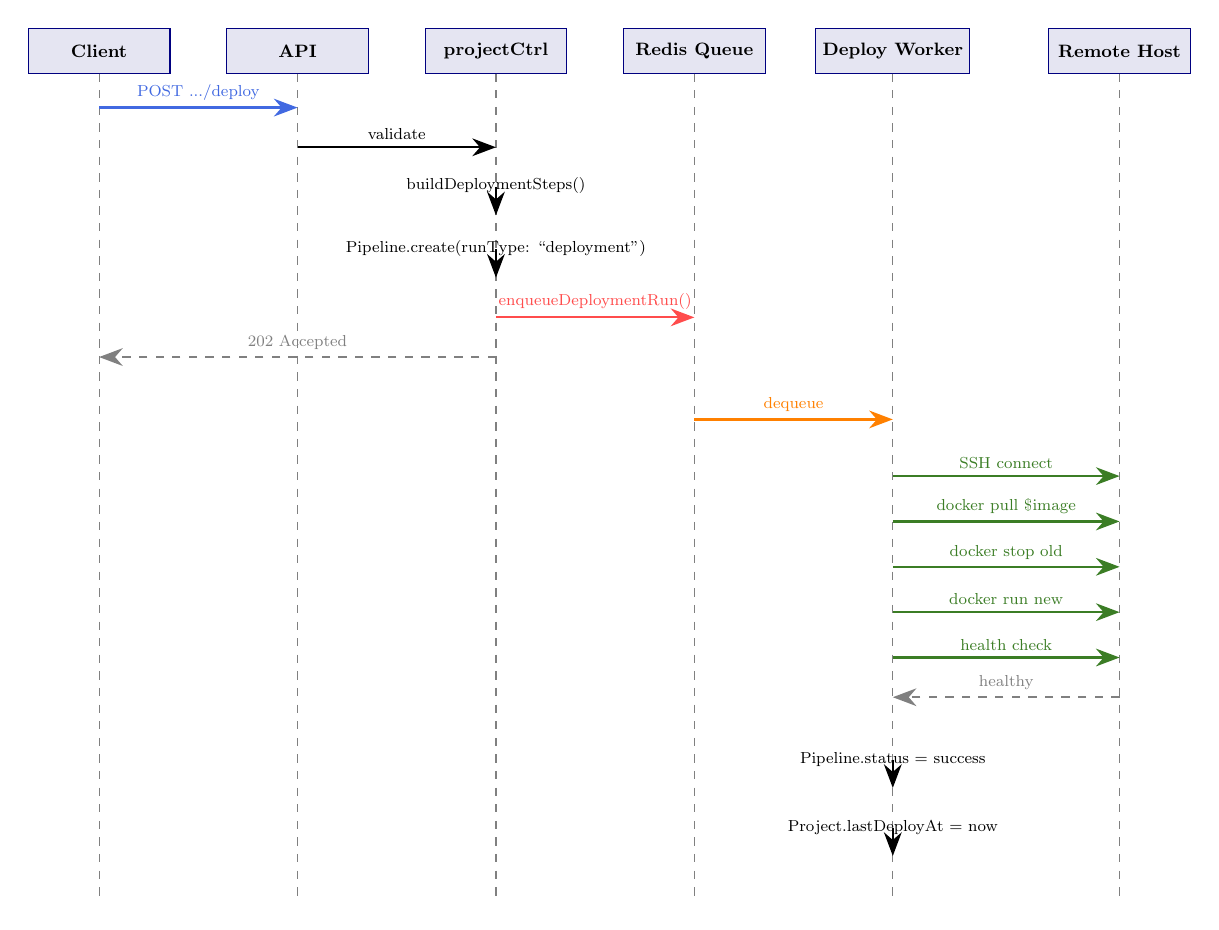
\begin{tikzpicture}[scale=0.72, transform shape]

  \node[seqobj] (client) at (0, 0) {Client};
  \node[seqobj] (api) at (3.5, 0) {API};
  \node[seqobj] (ctrl) at (7, 0) {projectCtrl};
  \node[seqobj] (queue) at (10.5, 0) {Redis Queue};
  \node[seqobj] (worker) at (14, 0) {Deploy Worker};
  \node[seqobj] (host) at (18, 0) {Remote Host};

  \foreach \x in {0, 3.5, 7, 10.5, 14, 18}
    \draw[dashed, gray] (\x, -0.4) -- (\x, -15);

  \draw[arrow, RoyalBlue] (0, -1) -- node[above, font=\footnotesize] {POST .../deploy} (3.5, -1);
  \draw[arrow] (3.5, -1.7) -- node[above, font=\footnotesize] {validate} (7, -1.7);
  \draw[arrow] (7, -2.4) -- node[above, font=\footnotesize] {buildDeploymentSteps()} (7, -2.9);
  \draw[arrow] (7, -3.5) -- node[above, font=\footnotesize] {Pipeline.create(runType: ``deployment'')} (7, -4);
  \draw[arrow, red!70] (7, -4.7) -- node[above, font=\footnotesize] {enqueueDeploymentRun()} (10.5, -4.7);
  \draw[dashedarrow, gray] (7, -5.4) -- node[above, font=\footnotesize] {202 Accepted} (0, -5.4);

  \draw[arrow, orange] (10.5, -6.5) -- node[above, font=\footnotesize] {dequeue} (14, -6.5);

  \draw[arrow, OliveGreen] (14, -7.5) -- node[above, font=\footnotesize] {SSH connect} (18, -7.5);
  \draw[arrow, OliveGreen] (14, -8.3) -- node[above, font=\footnotesize] {docker pull \$image} (18, -8.3);
  \draw[arrow, OliveGreen] (14, -9.1) -- node[above, font=\footnotesize] {docker stop old} (18, -9.1);
  \draw[arrow, OliveGreen] (14, -9.9) -- node[above, font=\footnotesize] {docker run new} (18, -9.9);
  \draw[arrow, OliveGreen] (14, -10.7) -- node[above, font=\footnotesize] {health check} (18, -10.7);
  \draw[dashedarrow, gray] (18, -11.4) -- node[above, font=\footnotesize] {healthy} (14, -11.4);

  \draw[arrow] (14, -12.5) -- node[above, font=\footnotesize] {Pipeline.status = success} (14, -13);
  \draw[arrow] (14, -13.7) -- node[above, font=\footnotesize] {Project.lastDeployAt = now} (14, -14.2);

\end{tikzpicture}
\caption{Deployment Execution Sequence Diagram}
\label{fig:seq-deploy}
\end{figure}

\section{Webhook-Triggered Pipeline}

\begin{figure}[H]
\centering
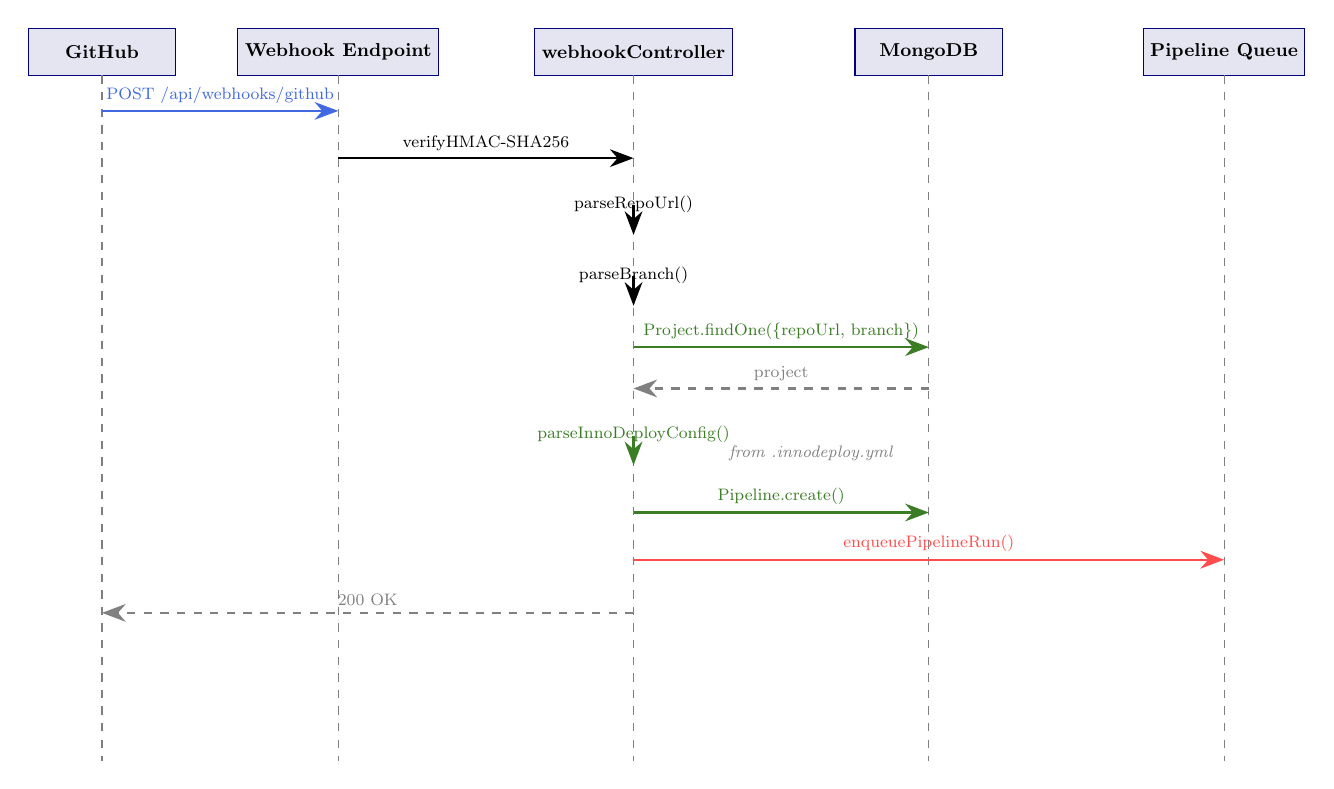
\begin{tikzpicture}[scale=0.75, transform shape]

  \node[seqobj] (github) at (0, 0) {GitHub};
  \node[seqobj] (api) at (4, 0) {Webhook Endpoint};
  \node[seqobj] (ctrl) at (9, 0) {webhookController};
  \node[seqobj] (db) at (14, 0) {MongoDB};
  \node[seqobj] (queue) at (19, 0) {Pipeline Queue};

  \foreach \x in {0, 4, 9, 14, 19}
    \draw[dashed, gray] (\x, -0.4) -- (\x, -12);

  \draw[arrow, RoyalBlue] (0, -1) -- node[above, font=\footnotesize] {POST /api/webhooks/github} (4, -1);
  \draw[arrow] (4, -1.8) -- node[above, font=\footnotesize] {verifyHMAC-SHA256} (9, -1.8);
  \draw[arrow] (9, -2.6) -- node[above, font=\footnotesize] {parseRepoUrl()} (9, -3.1);
  \draw[arrow] (9, -3.8) -- node[above, font=\footnotesize] {parseBranch()} (9, -4.3);

  \draw[arrow, OliveGreen] (9, -5) -- node[above, font=\footnotesize] {Project.findOne(\{repoUrl, branch\})} (14, -5);
  \draw[dashedarrow, gray] (14, -5.7) -- node[above, font=\footnotesize] {project} (9, -5.7);

  \draw[arrow, OliveGreen] (9, -6.5) -- node[above, font=\footnotesize] {parseInnoDeployConfig()} (9, -7);
  \node[font=\footnotesize\itshape, gray] at (12, -6.8) {from .innodeploy.yml};

  \draw[arrow, OliveGreen] (9, -7.8) -- node[above, font=\footnotesize] {Pipeline.create()} (14, -7.8);
  \draw[arrow, red!70] (9, -8.6) -- node[above, font=\footnotesize] {enqueuePipelineRun()} (19, -8.6);

  \draw[dashedarrow, gray] (9, -9.5) -- node[above, font=\footnotesize] {200 OK} (0, -9.5);

\end{tikzpicture}
\caption{Webhook-Triggered Pipeline Sequence Diagram}
\label{fig:seq-webhook}
\end{figure}

\section{Token Refresh Flow}

\begin{figure}[H]
\centering
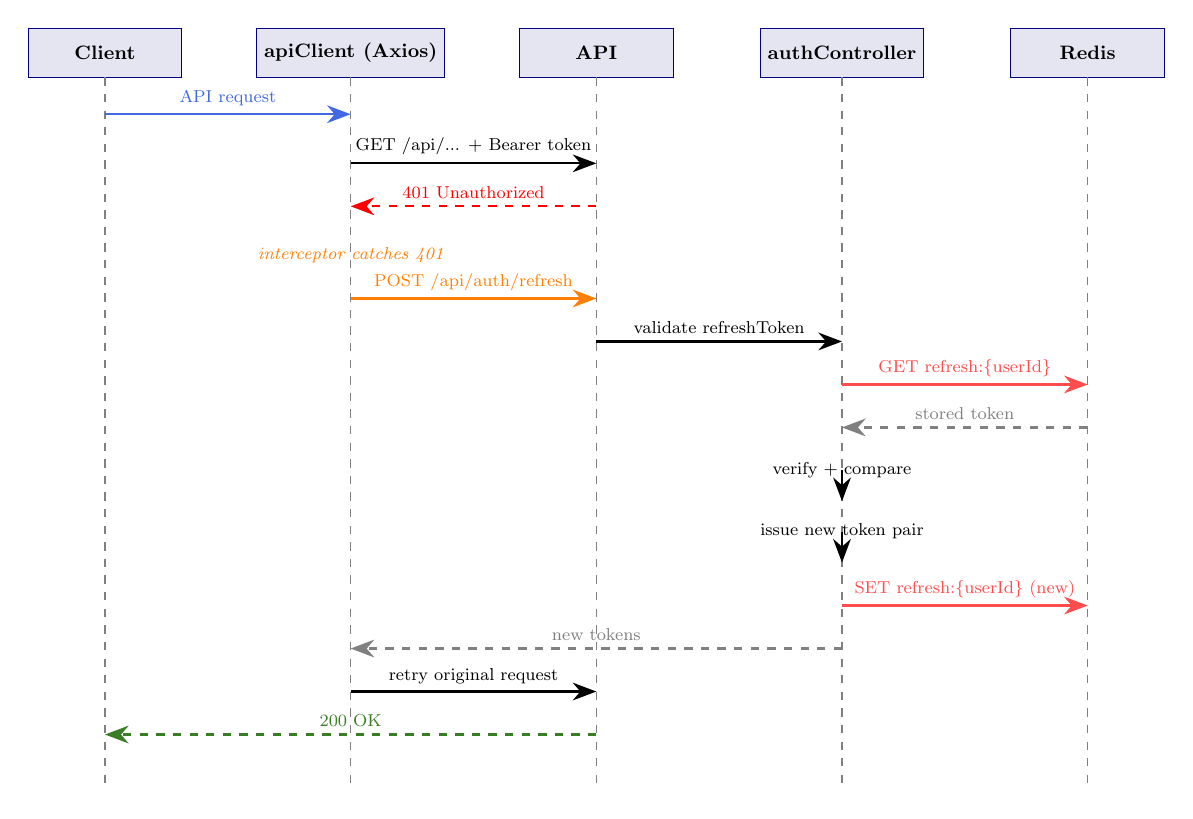
\begin{tikzpicture}[scale=0.78, transform shape]

  \node[seqobj] (client) at (0, 0) {Client};
  \node[seqobj] (axios) at (4, 0) {apiClient (Axios)};
  \node[seqobj] (api) at (8, 0) {API};
  \node[seqobj] (auth) at (12, 0) {authController};
  \node[seqobj] (redis) at (16, 0) {Redis};

  \foreach \x in {0, 4, 8, 12, 16}
    \draw[dashed, gray] (\x, -0.4) -- (\x, -12);

  \draw[arrow, RoyalBlue] (0, -1) -- node[above, font=\footnotesize] {API request} (4, -1);
  \draw[arrow] (4, -1.8) -- node[above, font=\footnotesize] {GET /api/... + Bearer token} (8, -1.8);
  \draw[dashedarrow, red] (8, -2.5) -- node[above, font=\footnotesize] {401 Unauthorized} (4, -2.5);

  \node[font=\footnotesize\itshape, orange] at (4, -3.3) {interceptor catches 401};

  \draw[arrow, orange] (4, -4) -- node[above, font=\footnotesize] {POST /api/auth/refresh} (8, -4);
  \draw[arrow] (8, -4.7) -- node[above, font=\footnotesize] {validate refreshToken} (12, -4.7);
  \draw[arrow, red!70] (12, -5.4) -- node[above, font=\footnotesize] {GET refresh:\{userId\}} (16, -5.4);
  \draw[dashedarrow, gray] (16, -6.1) -- node[above, font=\footnotesize] {stored token} (12, -6.1);

  \draw[arrow] (12, -6.8) -- node[above, font=\footnotesize] {verify + compare} (12, -7.3);
  \draw[arrow] (12, -7.8) -- node[above, font=\footnotesize] {issue new token pair} (12, -8.3);
  \draw[arrow, red!70] (12, -9) -- node[above, font=\footnotesize] {SET refresh:\{userId\} (new)} (16, -9);

  \draw[dashedarrow, gray] (12, -9.7) -- node[above, font=\footnotesize] {new tokens} (4, -9.7);
  \draw[arrow] (4, -10.4) -- node[above, font=\footnotesize] {retry original request} (8, -10.4);
  \draw[dashedarrow, OliveGreen] (8, -11.1) -- node[above, font=\footnotesize] {200 OK} (0, -11.1);

\end{tikzpicture}
\caption{Token Refresh Sequence Diagram}
\label{fig:seq-refresh}
\end{figure}


% ══════════════════════════════════════════════════════════════════════════
%  CHAPTER 7 – IMPLEMENTATION
% ══════════════════════════════════════════════════════════════════════════
\chapter{Implementation}

\section{Backend REST API}

\subsection{API Endpoint Summary}

The backend exposes approximately 60 RESTful endpoints organised across 12 route files:

\begin{longtable}{l|l|p{7cm}}
\caption{Complete API Endpoint Reference} \label{tab:api-endpoints} \\
\toprule
\textbf{Method} & \textbf{Path} & \textbf{Description} \\
\midrule
\endfirsthead
\toprule
\textbf{Method} & \textbf{Path} & \textbf{Description} \\
\midrule
\endhead
\midrule
\multicolumn{3}{r}{\textit{Continued on next page}} \\
\endfoot
\bottomrule
\endlastfoot

\multicolumn{3}{c}{\textbf{Authentication}} \\
\midrule
POST & /api/auth/register & User registration \\
POST & /api/auth/login & Email/password login \\
POST & /api/auth/refresh & Token refresh \\
POST & /api/auth/logout & Revoke refresh token \\
POST & /api/auth/forgot-password & Initiate password reset \\
POST & /api/auth/reset-password & Complete password reset \\
GET & /api/auth/google & Google OAuth initiation \\
GET & /api/auth/google/callback & Google OAuth callback \\
GET & /api/auth/github & GitHub OAuth initiation \\
GET & /api/auth/github/callback & GitHub OAuth callback \\
\midrule

\multicolumn{3}{c}{\textbf{Projects}} \\
\midrule
GET & /api/projects & List all projects \\
POST & /api/projects & Create project \\
GET & /api/projects/:id & Get project details \\
PATCH & /api/projects/:id & Update project \\
DELETE & /api/projects/:id & Delete project (cascade) \\
POST & /api/projects/:id/envs & Create environment \\
PATCH & /api/projects/:id/envs/:env & Update environment \\
DELETE & /api/projects/:id/envs/:env & Delete environment \\
POST & /api/projects/:id/envs/:env/secrets & Upsert secret \\
POST & /api/projects/:id/deploy & Trigger deployment \\
POST & /api/projects/:id/rollback & Rollback deployment \\
GET & /api/projects/:id/deploy/history & Deployment history \\
\midrule

\multicolumn{3}{c}{\textbf{Pipelines}} \\
\midrule
POST & /api/projects/:id/pipelines & Trigger pipeline \\
GET & /api/projects/:id/pipelines & List runs \\
GET & /api/pipelines/:runId & Get run details \\
POST & /api/pipelines/:runId/cancel & Cancel running pipeline \\
GET & /api/pipelines/:runId/logs/:stage & Get stage logs \\
GET & /api/pipelines/:runId/stream & SSE stream \\
\midrule

\multicolumn{3}{c}{\textbf{Hosts}} \\
\midrule
GET & /api/hosts & List hosts \\
POST & /api/hosts & Create host \\
GET & /api/hosts/:id & Get host \\
PATCH & /api/hosts/:id & Update host \\
DELETE & /api/hosts/:id & Remove host \\
POST & /api/hosts/test-connection & Test draft SSH \\
POST & /api/hosts/:id/test-connection & Test existing SSH \\
\midrule

\multicolumn{3}{c}{\textbf{Monitoring}} \\
\midrule
GET & /api/projects/:id/metrics & Get metrics \\
GET & /api/projects/:id/logs & Get logs \\
GET & /api/projects/:id/status & Health status \\
\midrule

\multicolumn{3}{c}{\textbf{Alerts}} \\
\midrule
GET & /api/alerts & List alerts \\
POST & /api/alerts & Create alert \\
PATCH & /api/alerts/:id/acknowledge & Acknowledge \\
PATCH & /api/alerts/:id/resolve & Resolve \\
DELETE & /api/alerts/:id & Delete alert \\
GET & /api/alerts/rules & Get rules \\
PUT & /api/alerts/rules & Update rules \\
POST & /api/alerts/rules/test-notification & Test notification \\
\midrule

\multicolumn{3}{c}{\textbf{Webhooks}} \\
\midrule
POST & /api/webhooks/github & GitHub webhook \\
POST & /api/webhooks/gitlab & GitLab webhook \\
POST & /api/webhooks/bitbucket & Bitbucket webhook \\

\end{longtable}

\subsection{Request Validation with Zod}

All incoming requests are validated at the route level using Zod schemas. Example:

\begin{lstlisting}[language=JavaScript, caption={Zod Schema for Pipeline Trigger}]
const triggerPipelineSchema = z.object({
  version:     z.string().min(1).max(50),
  strategy:    z.enum(["rolling","blue-green","canary","recreate"])
                .optional(),
  branch:      z.string().max(100).optional(),
  environment: z.string().min(1).max(50),
  config:      z.string().max(50000).optional(),
  steps:       z.array(z.object({
    name:      z.string().min(1).max(100),
    command:   z.string().min(1).max(5000),
    image:     z.string().max(200).optional(),
    retries:   z.number().int().min(0).max(5).optional(),
    timeoutMs: z.number().int().min(1000).optional()
  })).max(20).optional()
});
\end{lstlisting}

\subsection{Security Implementation}

\begin{itemize}[noitemsep]
  \item \textbf{Password hashing}: bcrypt with 12 salt rounds (pre-save hook on User model).
  \item \textbf{JWT}: Access token (short-lived) + Refresh token (7-day, stored in Redis for server-side revocation).
  \item \textbf{Secret encryption}: Project environment secrets encrypted with AES before MongoDB storage.
  \item \textbf{Rate limiting}: Auth endpoints limited to 20 requests per 15 minutes; password reset limited to 5 per 15 minutes; webhooks limited to 30 per minute.
  \item \textbf{Security headers}: Helmet.js middleware applies CSP, HSTS, X-Frame-Options, etc.
  \item \textbf{CORS}: Origin validation against configured \texttt{CLIENT\_URL}.
  \item \textbf{Webhook verification}: HMAC-SHA256 for GitHub, token verification for GitLab, signature verification for Bitbucket.
\end{itemize}

\section{Worker Subsystem}

\subsection{Pipeline Runner}

The pipeline runner is the core execution engine:

\begin{enumerate}[noitemsep]
  \item Polls the Redis pipeline queue using \texttt{BLPOP} (blocking pop).
  \item For each step, creates an isolated Docker container from the specified image (default: \texttt{node:20-alpine}).
  \item Clones the Git repository into the container workspace.
  \item Executes the step command, capturing stdout and stderr.
  \item Supports configurable timeouts (default 10 minutes) and retries per step.
  \item Publishes progress events to Redis channels for real-time streaming.
  \item On completion, updates the Pipeline document with final status and duration.
  \item Concurrency is configurable via \texttt{PIPELINE\_RUNNER\_CONCURRENCY} (default: 1).
\end{enumerate}

\subsection{Deploy Worker}

The deploy worker handles deployment orchestration:

\begin{enumerate}[noitemsep]
  \item Dequeues deployment jobs from the Redis deployment queue.
  \item Establishes SSH connection to the target host using SSH2.
  \item Executes deployment steps: image pull, container stop, container start, health check.
  \item Supports four strategies: \textbf{rolling} (incremental replacement), \textbf{blue-green} (stack switch), \textbf{canary} (gradual traffic shift), and \textbf{recreate} (full restart).
  \item Updates Pipeline status and Project deployment timestamp on completion.
\end{enumerate}

\subsection{Monitor Worker}

The monitoring worker continuously collects infrastructure metrics:

\begin{enumerate}[noitemsep]
  \item Periodically polls Docker containers for CPU, memory, network, and disk metrics.
  \item Executes health probes (HTTP, TCP, or container-based) to determine service availability.
  \item Stores metrics in the Metric collection.
  \item Publishes real-time metric updates to Redis monitoring channels.
  \item Feeds data to the alert rules engine for threshold evaluation.
\end{enumerate}

\subsection{Log Collector}

\begin{enumerate}[noitemsep]
  \item Aggregates Docker container logs via the Docker API.
  \item Stores logs in the Log collection with structured metadata.
  \item Publishes log entries to Redis log channels for real-time streaming.
  \item Supports TTL-based auto-expiration for storage management.
\end{enumerate}

\section{Frontend Dashboard}

\subsection{State Management}

The dashboard uses \textbf{Zustand} for global auth state and \textbf{React Query (TanStack Query)} for server state:

\begin{lstlisting}[language=JavaScript, caption={Zustand Auth Store}]
const useAuthStore = create((set) => ({
  user: null,
  accessToken: null,
  refreshToken: null,
  isAuthenticated: false,
  setAuth: (data) => set({
    user: data.user,
    accessToken: data.accessToken,
    refreshToken: data.refreshToken,
    isAuthenticated: true
  }),
  clearAuth: () => set({
    user: null, accessToken: null,
    refreshToken: null, isAuthenticated: false
  }),
  hydrate: () => { /* restore from localStorage */ }
}));
\end{lstlisting}

\subsection{API Client with Token Refresh}

The Axios-based API client implements automatic token refresh:

\begin{itemize}[noitemsep]
  \item Request interceptor injects the Bearer token from the auth store.
  \item Response interceptor catches 401 errors and attempts token refresh.
  \item On successful refresh, retries the original request transparently.
  \item On refresh failure, clears auth state and redirects to login.
\end{itemize}

\subsection{Real-Time WebSocket Integration}

The \texttt{useSocket} hook manages WebSocket connections:

\begin{itemize}[noitemsep]
  \item Connects to the WebSocket gateway with JWT authentication.
  \item Supports subscription to project-scoped monitoring channels.
  \item Handles reconnection with exponential backoff.
  \item Routes incoming messages to the appropriate UI components.
\end{itemize}

\section{CLI Tool}

The \texttt{innodeploy} CLI provides terminal-based access to all major platform features:

\begin{lstlisting}[language=bash, caption={CLI Command Examples}]
# Authenticate
innodeploy login

# Project management
innodeploy projects list
innodeploy projects create my-app

# Deployment
innodeploy deploy my-app --env production
innodeploy rollback my-app --env production

# Pipeline
innodeploy pipeline trigger my-app
innodeploy pipeline status <runId>

# Real-time logs
innodeploy logs my-app --env production --follow

# Scaffold config
innodeploy init
\end{lstlisting}

The CLI stores credentials in \texttt{\textasciitilde/.innodeploy-cli/config.json} and implements automatic token refresh on 401 responses, mirroring the dashboard's behaviour.

\section{Pipeline Configuration File}

Projects can define their CI/CD pipeline using a \texttt{.innodeploy.yml} file:

\begin{lstlisting}[language=yaml, caption={.innodeploy.yml Configuration Example}]
name: my-app-pipeline
strategy: rolling
environment: production
trigger:
  branch: main
steps:
  - name: Install dependencies
    command: npm ci
    image: node:20-alpine
    timeoutMs: 300000
  - name: Run tests
    command: npm test
    image: node:20-alpine
    retries: 2
  - name: Build
    command: npm run build
    image: node:20-alpine
  - name: Deploy
    command: ./scripts/deploy.sh
    timeoutMs: 600000
notifications:
  onSuccess: true
  onFailure: true
\end{lstlisting}


% ══════════════════════════════════════════════════════════════════════════
%  CHAPTER 8 – USER INTERFACE
% ══════════════════════════════════════════════════════════════════════════
\chapter{User Interface}

The InnoDeploy dashboard is built with Next.js 15, React 19, and Tailwind CSS, featuring a modern dark-themed design with cyan accent colour ({\color{innoprimary}\texttt{\#00D4AA}}). The interface supports three themes (light, dark, system) and three languages (English, French, Arabic).

\section{Login Page}

The login page provides multiple authentication methods: email/password, Google OAuth, and GitHub OAuth.

\begin{figure}[H]
\centering
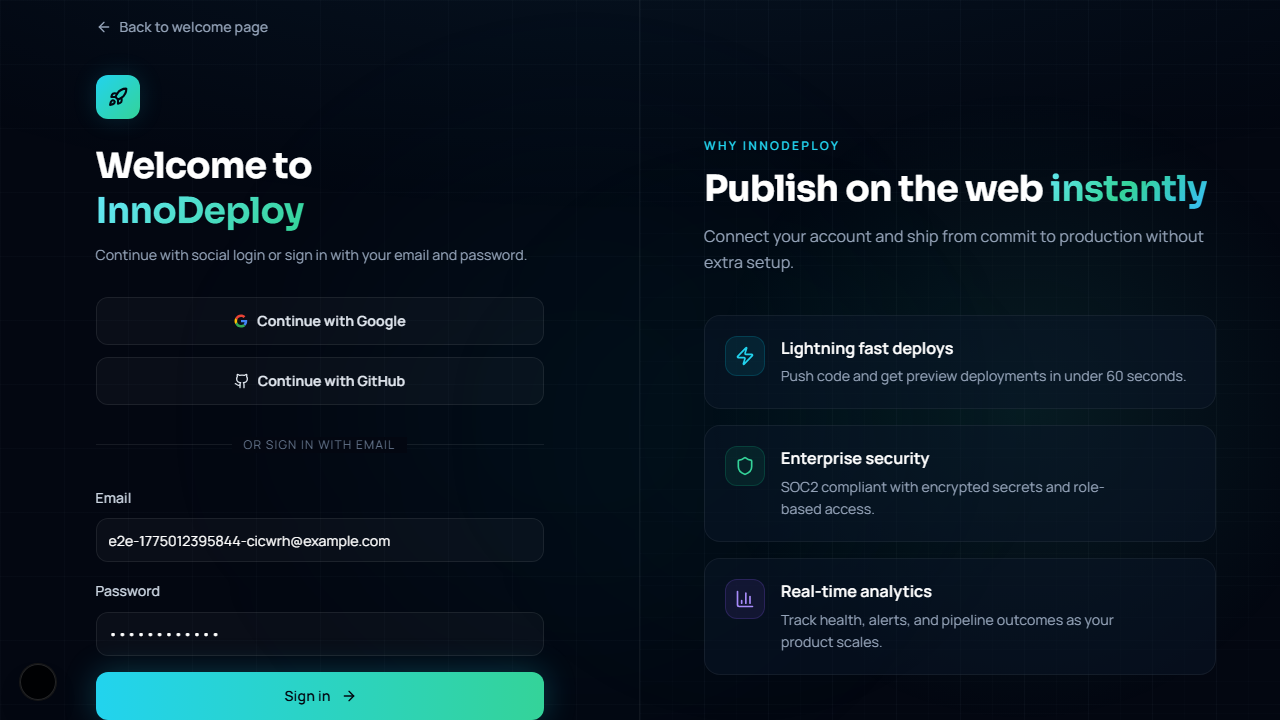
\includegraphics[width=0.95\textwidth]{images/login.png}
\caption{Login Page -- Email/Password and OAuth Authentication}
\label{fig:ui-login}
\end{figure}

Key features visible:
\begin{itemize}[noitemsep]
  \item Social login buttons (Google, GitHub) prominently displayed.
  \item Email and password form fields with validation.
  \item Right panel showcasing platform value propositions: \textit{Lightning fast deploys}, \textit{Enterprise security}, and \textit{Real-time analytics}.
  \item Theme toggle in the bottom-left corner.
\end{itemize}

\section{Registration Page}

New users register with name, email, password, and an optional organisation name:

\begin{figure}[H]
\centering
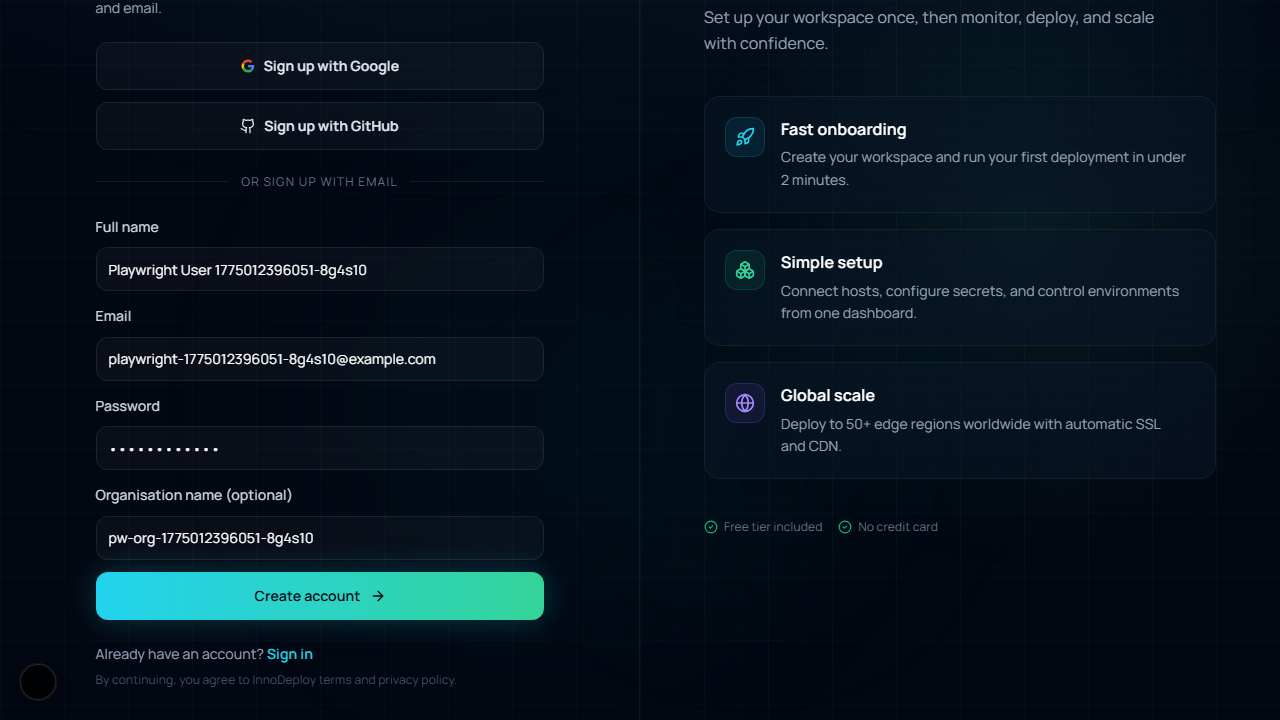
\includegraphics[width=0.95\textwidth]{images/register.png}
\caption{Registration Page -- Account Creation with Organisation}
\label{fig:ui-register}
\end{figure}

Key features:
\begin{itemize}[noitemsep]
  \item Social registration options (Google, GitHub).
  \item Organisation name field allows automatic workspace creation.
  \item ``Free tier included'' and ``No credit card'' trust indicators.
  \item Right panel highlights: \textit{Fast onboarding}, \textit{Simple setup}, \textit{Global scale}.
\end{itemize}

\section{Dashboard Overview}

The main dashboard page provides a high-level summary of the organisation's resources:

\begin{itemize}[noitemsep]
  \item \textbf{Stats cards}: Total projects, active deployments, hosts online, open alerts.
  \item \textbf{14-day trend charts}: New users, projects created, pipeline runs, alerts triggered.
  \item \textbf{Recent activity}: Latest pipeline runs with status indicators.
  \item \textbf{Sidebar navigation}: Projects, Hosts, Pipelines, Monitoring, Alerts, Logs, Settings, Documentation.
\end{itemize}

\section{Projects Page}

The projects listing page displays all projects for the current organisation:

\begin{figure}[H]
\centering
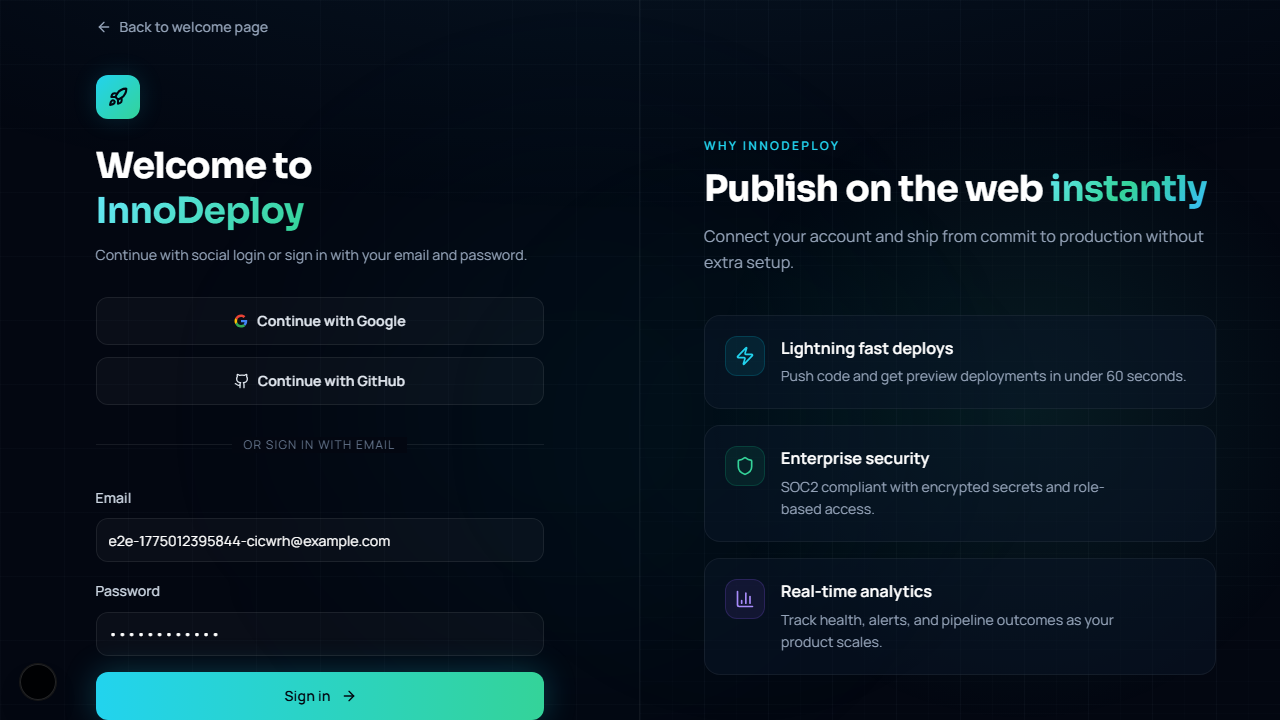
\includegraphics[width=0.95\textwidth]{images/projects.png}
\caption{Projects Page -- Project List with Status}
\label{fig:ui-projects}
\end{figure}

Features:
\begin{itemize}[noitemsep]
  \item Project cards showing name, repository URL, status, and last deploy time.
  \item Quick-action buttons for deployment, pipeline trigger, and settings.
  \item Environment badges showing configured deployment targets.
\end{itemize}

\section{Key UI Component Summary}

\begin{table}[H]
\centering
\caption{Dashboard UI Components}
\label{tab:ui-components}
\begin{tabularx}{\textwidth}{l|X}
\toprule
\textbf{Page/Component} & \textbf{Description} \\
\midrule
Landing Page & Marketing page with hero section, feature cards, pricing, and testimonials \\
Dashboard & Admin overview with stats, trends, and recent activity \\
Projects List & Card grid of all projects with status and quick actions \\
Project Detail & Environments, secrets, deployment history, and settings \\
New Project & Form wizard for creating a project from a Git repository \\
Pipeline Detail & Step-by-step execution view with live log output and status \\
Hosts Page & Host list with SSH status, resource usage, and container info \\
Monitoring & Real-time charts (CPU, memory, disk, latency) using Recharts \\
Logs & Terminal-style log viewer (xterm.js) with filters and search \\
Alerts & Alert list with severity badges, acknowledge/resolve actions \\
Settings & Organisation profile, members, notifications, Docker registry, API keys \\
Admin Dashboard & System-wide stats with user management (owner/admin only) \\
Docs & Built-in documentation viewer \\
Support & Help and support page \\
\bottomrule
\end{tabularx}
\end{table}


% ══════════════════════════════════════════════════════════════════════════
%  CHAPTER 9 – DEPLOYMENT
% ══════════════════════════════════════════════════════════════════════════
\chapter{Deployment}

\section{Deployment Diagram}

\begin{figure}[H]
\centering
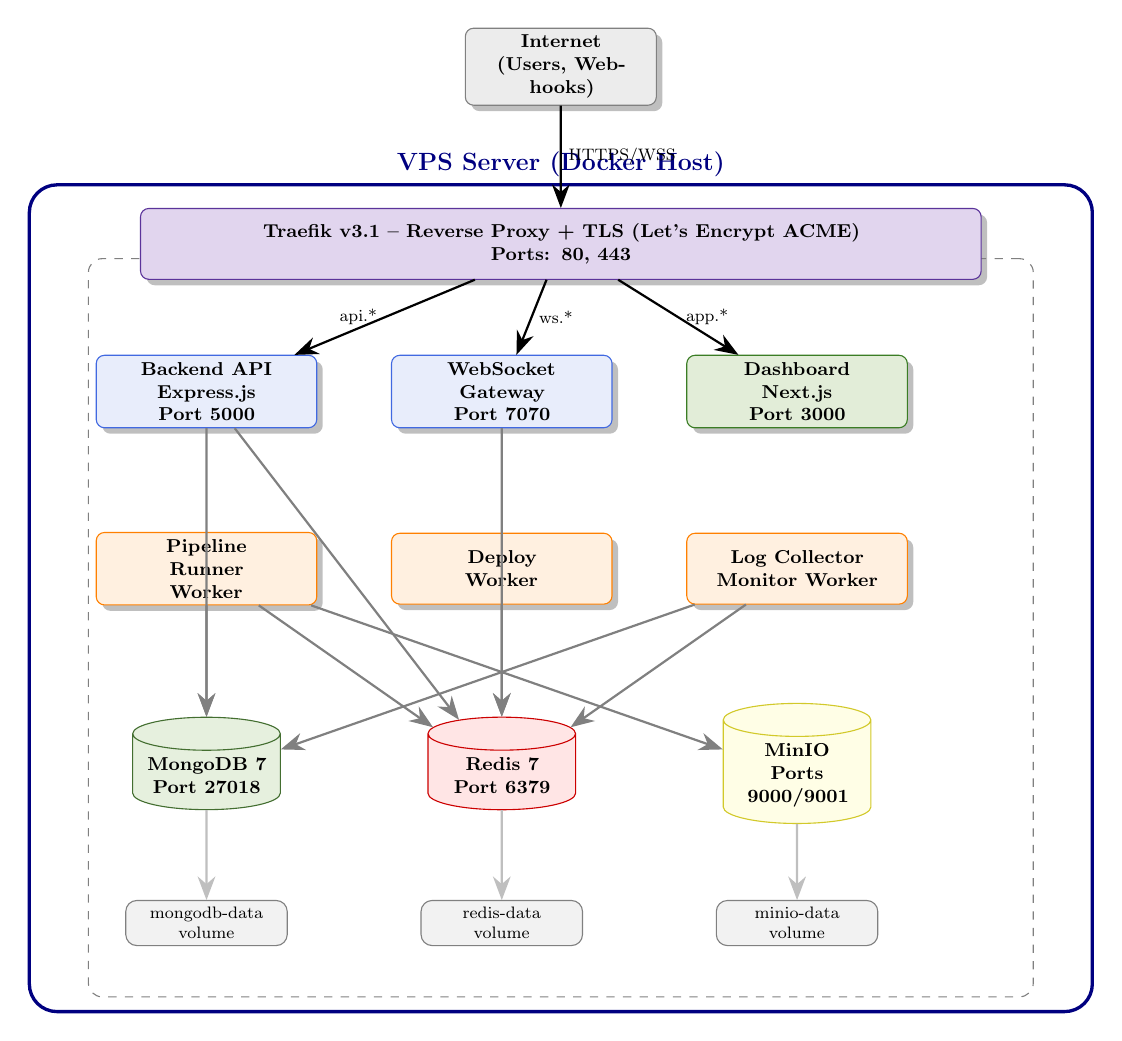
\begin{tikzpicture}[node distance=1.5cm and 2cm, scale=0.75, transform shape]

  % VPS Node
  \node[draw=NavyBlue, very thick, rounded corners=10pt,
        minimum width=18cm, minimum height=14cm,
        label={[font=\large\bfseries\color{NavyBlue}]above:VPS Server (Docker Host)}] (vps) at (8, -5) {};

  % Docker Network
  \node[draw=gray, dashed, rounded corners=5pt,
        minimum width=16cm, minimum height=12.5cm,
        label={[font=\small\itshape]above:innodeploy-net (Docker Bridge Network)}] at (8, -5.5) {};

  % Traefik
  \node[component, fill=RoyalPurple!15, draw=RoyalPurple, text width=14cm, minimum height=1.2cm]
    (traefik) at (8, 1) {Traefik v3.1 -- Reverse Proxy + TLS (Let's Encrypt ACME)\\Ports: 80, 443};

  % Application Services
  \node[component, fill=RoyalBlue!12, draw=RoyalBlue, text width=3.5cm]
    (api) at (2, -1.5) {Backend API\\Express.js\\Port 5000};
  \node[component, fill=RoyalBlue!12, draw=RoyalBlue, text width=3.5cm]
    (wsgateway) at (7, -1.5) {WebSocket\\Gateway\\Port 7070};
  \node[component, fill=OliveGreen!12, draw=OliveGreen, text width=3.5cm]
    (dash) at (12, -1.5) {Dashboard\\Next.js\\Port 3000};

  % Workers
  \node[component, fill=orange!12, draw=orange, text width=3.5cm]
    (pr) at (2, -4.5) {Pipeline\\Runner\\Worker};
  \node[component, fill=orange!12, draw=orange, text width=3.5cm]
    (dw) at (7, -4.5) {Deploy\\Worker};
  \node[component, fill=orange!12, draw=orange, text width=3.5cm]
    (lcollector) at (12, -4.5) {Log Collector\\Monitor Worker};

  % Data Services
  \node[database, minimum width=2.5cm] (mongo) at (2, -8) {MongoDB 7\\Port 27018};
  \node[database, fill=red!10, draw=red!80!black, minimum width=2.5cm]
    (redis) at (7, -8) {Redis 7\\Port 6379};
  \node[database, fill=yellow!10, draw=yellow!80!black, minimum width=2.5cm]
    (minio) at (12, -8) {MinIO\\Ports 9000/9001};

  % Volumes
  \node[rectangle, draw=gray, fill=gray!10, rounded corners, text width=2.5cm, text centered, font=\footnotesize]
    (v1) at (2, -10.5) {mongodb-data\\volume};
  \node[rectangle, draw=gray, fill=gray!10, rounded corners, text width=2.5cm, text centered, font=\footnotesize]
    (v2) at (7, -10.5) {redis-data\\volume};
  \node[rectangle, draw=gray, fill=gray!10, rounded corners, text width=2.5cm, text centered, font=\footnotesize]
    (v3) at (12, -10.5) {minio-data\\volume};

  % External
  \node[server, fill=gray!15, draw=gray] (internet) at (8, 4) {Internet\\(Users, Webhooks)};

  % Connections
  \draw[arrow] (internet) -- node[right, font=\footnotesize] {HTTPS/WSS} (traefik);
  \draw[arrow] (traefik) -- node[left, font=\footnotesize] {api.*} (api);
  \draw[arrow] (traefik) -- node[right, font=\footnotesize] {ws.*} (wsgateway);
  \draw[arrow] (traefik) -- node[right, font=\footnotesize] {app.*} (dash);

  \draw[arrow, gray] (api) -- (mongo);
  \draw[arrow, gray] (api) -- (redis);
  \draw[arrow, gray] (pr) -- (mongo);
  \draw[arrow, gray] (pr) -- (redis);
  \draw[arrow, gray] (dw) -- (redis);
  \draw[arrow, gray] (wsgateway) -- (redis);
  \draw[arrow, gray] (pr) -- (minio);
  \draw[arrow, gray] (lcollector) -- (mongo);
  \draw[arrow, gray] (lcollector) -- (redis);

  \draw[arrow, gray!50] (mongo) -- (v1);
  \draw[arrow, gray!50] (redis) -- (v2);
  \draw[arrow, gray!50] (minio) -- (v3);

\end{tikzpicture}
\caption{UML Deployment Diagram}
\label{fig:deployment-diagram}
\end{figure}

\section{Docker Compose Configuration}

The entire platform is orchestrated using Docker Compose with 8 services:

\begin{table}[H]
\centering
\caption{Docker Compose Services}
\label{tab:docker-services}
\begin{tabularx}{\textwidth}{l|l|X}
\toprule
\textbf{Service} & \textbf{Image/Base} & \textbf{Role} \\
\midrule
traefik & traefik:v3.1 & Reverse proxy with auto-TLS via Let's Encrypt \\
backend & Custom (Dockerfile) & Express.js API server \\
websocket & Custom (Dockerfile) & WebSocket gateway for real-time updates \\
dashboard & Custom (Dockerfile) & Next.js frontend application \\
mongodb & mongo:7 & Primary database \\
redis & redis:7 & Cache, queues, pub/sub, token storage \\
minio & minio & S3-compatible artifact storage \\
pipeline-runner & Custom (Dockerfile) & Background pipeline execution worker \\
deploy-worker & Custom (Dockerfile) & Background deployment execution worker \\
\bottomrule
\end{tabularx}
\end{table}

\section{Traefik Configuration}

Traefik provides:
\begin{itemize}[noitemsep]
  \item \textbf{Automatic HTTPS}: Let's Encrypt ACME with HTTP-01 challenge.
  \item \textbf{Service discovery}: Docker labels for automatic route registration.
  \item \textbf{Rate limiting}: Middleware for API endpoint protection.
  \item \textbf{Domain routing}: \texttt{api.*} $\rightarrow$ backend, \texttt{ws.*} $\rightarrow$ websocket, \texttt{app.*} $\rightarrow$ dashboard.
  \item \textbf{WebSocket support}: Transparent upgrade for the WebSocket gateway.
\end{itemize}

\section{Environment Variables}

\begin{table}[H]
\centering
\caption{Key Environment Variables}
\label{tab:env-vars}
\begin{tabularx}{\textwidth}{l|l|X}
\toprule
\textbf{Variable} & \textbf{Default} & \textbf{Purpose} \\
\midrule
PORT & 5000 & Backend API port \\
MONGO\_URI & localhost:27017 & MongoDB connection string \\
REDIS\_URL & localhost:6379 & Redis connection string \\
JWT\_SECRET & -- & JWT signing secret \\
JWT\_REFRESH\_SECRET & -- & Refresh token signing secret \\
CLIENT\_URL & -- & CORS allowed origin \\
GOOGLE\_CLIENT\_ID & -- & Google OAuth credentials \\
GITHUB\_CLIENT\_ID & -- & GitHub OAuth credentials \\
WS\_PORT & 7070 & WebSocket gateway port \\
PIPELINE\_RUNNER\_CONCURRENCY & 1 & Parallel pipeline slots \\
PIPELINE\_STEP\_TIMEOUT\_MS & 600000 & Step execution timeout \\
LOG\_RETENTION\_DAYS & 30 & Log auto-expiration period \\
\bottomrule
\end{tabularx}
\end{table}

\section{Deployment Strategies Supported}

InnoDeploy supports four deployment strategies for application delivery:

\begin{table}[H]
\centering
\caption{Deployment Strategies}
\label{tab:deploy-strategies}
\begin{tabularx}{\textwidth}{l|X|l}
\toprule
\textbf{Strategy} & \textbf{Description} & \textbf{Downtime} \\
\midrule
\textbf{Rolling} & Incrementally replace old containers with new ones, performing health checks between each swap. & Zero \\
\textbf{Blue-Green} & Spin up a complete ``green'' environment, then switch traffic from ``blue'' to ``green'' atomically. & Near-zero \\
\textbf{Canary} & Gradually route increasing traffic percentages to the new version while monitoring for errors. & Zero \\
\textbf{Recreate} & Stop all old containers, then start new ones. Simple but causes brief downtime. Used for stateful services and rollbacks. & Brief \\
\bottomrule
\end{tabularx}
\end{table}


% ══════════════════════════════════════════════════════════════════════════
%  CHAPTER 10 – TESTING
% ══════════════════════════════════════════════════════════════════════════
\chapter{Testing}

\section{Testing Strategy}

InnoDeploy follows a multi-layer testing strategy:

\begin{figure}[H]
\centering
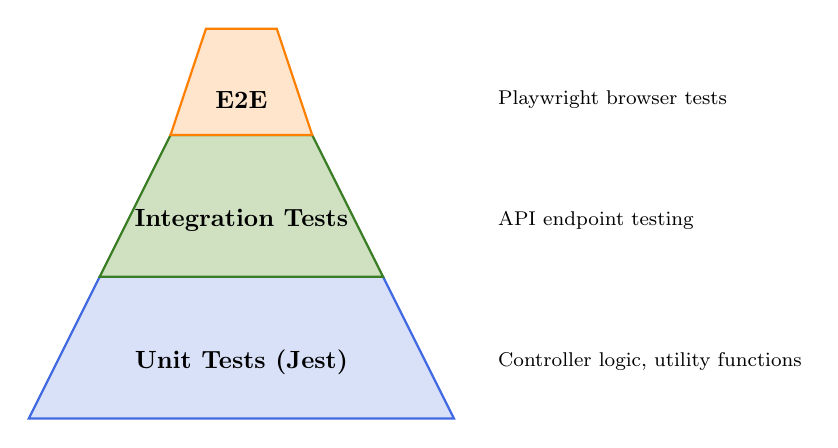
\begin{tikzpicture}[scale=0.9, transform shape]
  \draw[fill=RoyalBlue!20, draw=RoyalBlue, thick] (0,0) -- (6,0) -- (5,2) -- (1,2) -- cycle;
  \draw[fill=OliveGreen!20, draw=OliveGreen, thick] (1,2) -- (5,2) -- (4,4) -- (2,4) -- cycle;
  \draw[fill=orange!20, draw=orange, thick] (2,4) -- (4,4) -- (3.5,5.5) -- (2.5,5.5) -- cycle;

  \node[font=\bfseries] at (3, 0.8) {Unit Tests (Jest)};
  \node[font=\bfseries] at (3, 2.8) {Integration Tests};
  \node[font=\bfseries] at (3, 4.5) {E2E};

  \node[font=\footnotesize, right] at (6.5, 0.8) {Controller logic, utility functions};
  \node[font=\footnotesize, right] at (6.5, 2.8) {API endpoint testing};
  \node[font=\footnotesize, right] at (6.5, 4.5) {Playwright browser tests};
\end{tikzpicture}
\caption{Testing Pyramid}
\label{fig:testing-pyramid}
\end{figure}

\section{Unit Testing}

Unit tests are implemented using \textbf{Jest} for the backend:

\begin{itemize}[noitemsep]
  \item Controller functions tested in isolation with mocked models and services.
  \item Utility functions (encryption, token generation, validation) tested with edge cases.
  \item Test command: \texttt{npm test} with open handle detection.
\end{itemize}

\section{Integration Testing}

Integration tests verify API endpoints with a test database:

\begin{itemize}[noitemsep]
  \item HTTP requests against the Express app with supertest.
  \item Database seeding and cleanup between test suites.
  \item Authentication flow testing (register, login, refresh, logout).
  \item Project CRUD with environment and secret management.
\end{itemize}

\section{End-to-End Testing}

E2E tests use \textbf{Playwright} for browser-based testing of the dashboard:

\begin{itemize}[noitemsep]
  \item \textbf{Auth flows}: Registration with organisation creation, login with existing credentials.
  \item \textbf{Project management}: Creating projects, viewing project lists.
  \item \textbf{Pipeline execution}: Triggering pipelines from the project detail page.
  \item Chromium-based test execution with screenshot capture on failure.
  \item Configuration: \texttt{playwright.config.ts} with base URL and timeout settings.
\end{itemize}

\section{Pipeline End-to-End Testing}

A dedicated pipeline E2E test (\texttt{pipeline-e2e.js}) validates the complete pipeline lifecycle:

\begin{enumerate}[noitemsep]
  \item Register a test user and create an organisation.
  \item Create a project linked to a test repository.
  \item Trigger a pipeline run with custom steps.
  \item Poll the pipeline status until completion.
  \item Verify step outputs and final status.
  \item Clean up test data.
\end{enumerate}


% ══════════════════════════════════════════════════════════════════════════
%  CHAPTER 11 – CONCLUSION
% ══════════════════════════════════════════════════════════════════════════
\chapter{Conclusion}

\section{Summary of Contributions}

This project has successfully designed and implemented \textbf{InnoDeploy}, a comprehensive multi-tenant DevOps SaaS platform that addresses the fragmentation and complexity challenges in modern CI/CD tooling. The key contributions include:

\begin{enumerate}
  \item \textbf{Unified Platform}: A single platform consolidating CI/CD pipelines, deployment orchestration, monitoring, alerting, log aggregation, and secret management -- eliminating the need for multiple disparate tools.

  \item \textbf{Multi-Tenant Architecture}: Organisation-scoped resource isolation with four-tier RBAC (Owner, Admin, Developer, Viewer), plan-based limits, and complete audit trail with 90-day retention.

  \item \textbf{Pipeline Execution Engine}: Docker-container-isolated step execution with configurable timeouts, retries, and real-time progress streaming via SSE and WebSocket.

  \item \textbf{Multi-Strategy Deployment}: Support for rolling, blue-green, canary, and recreate deployment strategies with SSH-based execution on user-managed hosts.

  \item \textbf{Real-Time Monitoring}: WebSocket-based metric streaming with configurable alert thresholds and multi-channel notification dispatch (email, Slack, Discord, Expo push, webhooks).

  \item \textbf{Modern Dashboard}: A responsive Next.js dashboard with dark theme, internationalisation support, real-time data visualization, terminal-style log viewer, and Monaco code editor integration.

  \item \textbf{Developer-Friendly CLI}: A command-line tool providing full platform access with interactive prompts and automatic token refresh.

  \item \textbf{Production-Ready Infrastructure}: Docker Compose orchestration with Traefik reverse proxy, automatic TLS certificates, and persistent data volumes.
\end{enumerate}

\section{Technical Achievements}

\begin{itemize}[noitemsep]
  \item \textbf{9 data models} with comprehensive indexing and TTL-based data lifecycle management.
  \item \textbf{60+ REST API endpoints} with Zod schema validation and role-based access control.
  \item \textbf{4 background workers} (pipeline runner, deploy worker, monitor worker, log collector) with Redis-backed job queues.
  \item \textbf{15 service modules} handling notifications, queues, event streaming, and infrastructure integration.
  \item \textbf{3 webhook receivers} (GitHub, GitLab, Bitbucket) with cryptographic signature verification.
  \item \textbf{Multi-layer testing} with unit tests (Jest), integration tests, and E2E tests (Playwright).
\end{itemize}

\section{Limitations}

\begin{itemize}[noitemsep]
  \item \textbf{Single-node workers}: Pipeline and deploy workers run as single instances; horizontal scaling requires manual sharding.
  \item \textbf{Docker-only containers}: Pipeline steps currently only support Docker-based execution environments.
  \item \textbf{No built-in Git server}: The platform relies on external Git providers (GitHub, GitLab, Bitbucket).
\end{itemize}

\section{Future Work}

\begin{enumerate}
  \item \textbf{Kubernetes support}: Extend deployment targets to include Kubernetes clusters alongside Docker hosts.
  \item \textbf{Auto-scaling workers}: Implement dynamic worker scaling based on queue depth using Kubernetes HPA or Docker Swarm.
  \item \textbf{Plugin system}: Allow users to extend pipeline steps with custom plugins for specific build tools or deployment targets.
  \item \textbf{AI-powered insights}: Integrate machine learning for anomaly detection in metrics and predictive alerting.
  \item \textbf{Mobile application}: Develop native mobile apps for monitoring and alert management on-the-go.
  \item \textbf{GitOps integration}: Support declarative deployment configuration synced from Git repositories.
  \item \textbf{Multi-region deployment}: Enable geographic distribution of deployments across multiple VPS regions.
\end{enumerate}

\section{Final Remarks}

InnoDeploy demonstrates that a well-architected full-stack application can provide enterprise-grade DevOps capabilities in a unified, self-hosted package. The combination of real-time communication, containerised execution, multi-strategy deployment, and comprehensive observability creates a platform that is both powerful for production use and educational as an engineering project.

The project showcases modern best practices across the entire stack: event-driven architecture, JWT-based authentication with server-side revocation, Zod schema validation, Redis pub/sub for real-time features, and Docker Compose for reproducible deployment -- making it a comprehensive reference implementation for multi-tenant SaaS platform engineering.


% ══════════════════════════════════════════════════════════════════════════
%  APPENDICES
% ══════════════════════════════════════════════════════════════════════════
\appendix

\chapter{Project Directory Structure}

\begin{lstlisting}[basicstyle=\ttfamily\footnotesize, frame=none, numbers=none]
InnoDeploy/
|-- backend/
|   |-- Dockerfile
|   |-- package.json
|   `-- src/
|       |-- app.js              # Express setup
|       |-- server.js           # Bootstrap & shutdown
|       |-- config/
|       |   |-- db.js           # MongoDB connection
|       |   `-- redis.js        # Redis connection
|       |-- controllers/        # 11 controllers
|       |-- middleware/          # Auth, audit, validate, error
|       |-- models/             # 9 Mongoose models
|       |-- routes/             # 12 route files
|       |-- services/           # 15 service modules
|       |-- utils/              # Encryption, helpers
|       `-- workers/            # Worker entry points
|-- dashboard/
|   |-- Dockerfile
|   |-- package.json
|   |-- app/                    # Next.js pages (10 routes)
|   |-- components/             # 16 component directories
|   |-- hooks/                  # 3 custom hooks
|   |-- lib/                    # API client, socket, utils
|   |-- store/                  # Zustand auth store
|   |-- types/                  # TypeScript interfaces
|   `-- tests/                  # Playwright E2E tests
|-- cli/
|   |-- package.json
|   |-- bin/innodeploy.js       # CLI entry point
|   `-- src/                    # Config & prompts
|-- docker/
|   `-- docker-compose.yml      # 8-service orchestration
`-- docs/
    |-- architecture.md
    |-- PROJECT_STRUCTURE.md
    `-- README.md
\end{lstlisting}

\chapter{Glossary}

\begin{description}
  \item[API] Application Programming Interface -- a set of protocols for building software.
  \item[RBAC] Role-Based Access Control -- restricting system access based on user roles.
  \item[CI/CD] Continuous Integration / Continuous Deployment -- automated build and release pipeline.
  \item[JWT] JSON Web Token -- compact, URL-safe token for claims transmission.
  \item[SSE] Server-Sent Events -- HTTP-based one-way real-time data push.
  \item[WebSocket] Full-duplex communication protocol over a single TCP connection.
  \item[SaaS] Software as a Service -- cloud-delivered application model.
  \item[TLS] Transport Layer Security -- cryptographic protocol for secure communication.
  \item[ACME] Automatic Certificate Management Environment -- protocol for TLS certificate automation.
  \item[ODM] Object-Document Mapper -- maps objects to document database records.
  \item[TTL] Time to Live -- automatic expiration period for data records.
  \item[Pub/Sub] Publish/Subscribe -- messaging pattern for decoupled communication.
  \item[SSH] Secure Shell -- protocol for secure remote server access.
  \item[OAuth] Open Authorization -- delegated authentication protocol.
  \item[HMAC] Hash-based Message Authentication Code -- cryptographic signature for message integrity.
  \item[CORS] Cross-Origin Resource Sharing -- browser security mechanism for cross-domain requests.
\end{description}

\end{document}
